\newpage
\chapter{Measurement Higgs Self-coupling}
\label{HHyybb}

The aim of this thesis is to perform a measurement of the Higgs self-coupling using the full Run-2 data in the \HHyybb decay channel. Up to here, all the ingredients needed to reconstructed the \HHyybb events are presented in the previous chapters. This chapter describes the analysis strategy to measure the Higgs self-coupling.
%This chapter should include the HH analysis and \kl limits

\section{Data and simulation}
\label{HHyybb:Data&MC}
As mentioned before, the analysis uses the full Run-2 data recorded by ATLAS during 2015 to 2018 with a total of integrated luminosity of 139 $\pm$ 2.4 \ifb. The values of the integrated luminosity recorded in each year is shown in Table \ref{tab:HHyybb:Data&MC:Lumi} \cite{Lumi}. 
Similarly to $H\rightarrow\gamma\gamma$ analysis, the \HHyybb analysis relies on different set of di-photon triggers for each year. The trigger used for 2015-2016 requires at least two photons with $E_T$ is greater than 35 GeV for leading and 25 for the sub-leading photon passing the loose identification. The di-photon trigger used in 2017-2018 requires at least two photons with the same requirement of their transverses energy while for the identification the medium WP is used, due to the increasing rates. For boosted Higgs, two high momentum single-photon triggers available in 2018 were added in a logical OR with the di-photon, requiring a loose photon with an energy of 120 GeV and 140 GeV respectively. 
\begin{table}[ht]
    \centering
    \begin{tabular}{cc}
    \hline\hline
        Year & int. luminosity [\ifb]  \\ \hline
        2015-2016 & 36.21 \\
        2017      & 44.39 \\
        2018      & 58.45 \\
        \hline \hline
    \end{tabular}
    \caption{Integrated luminosity recorded by ATLAS in Run 2 per year of data taking.}
    \label{tab:HHyybb:Data&MC:Lumi}
\end{table}
The \HHyybb Monte Carlo (MC) are generated from two production mode the ggF HH and VBF HH. Events from ggF HH production were generated at NLO using the \textsc{Powheg-Box} v2 generator in the finite top-quark mass approximation with PDFLHC15 PDF set \cite{HH_FT, HH_Powheg, PDF4LHC}. The \textsc{PYTHIA} 8.2 is used for parton showering. Two samples are generated for \kl= 1 and \kl= 10. Events from the VBF HH production were generated at LO  using \textsc{MadGraph5\_aMC@NLO} \cite{HH_VBF} using the \texttt{NNPDF3.0nnlo} PDF set \cite{VBF_PDF} and \textsc{PYTHIA} for showering. \\

A reweighting procedure is developed to avoid generating MC samples for each \kl for both ggF and VBF. Truth level HH samples with 10M events are produced for \kl= 0, 1, 10 and 20 with specific HH decay mode. A linear combination of samples with \kl= 0, 1 and 20 derived from Equation \ref{eq:chap1:HH:XSEC:Param} is used to derive weight and \kl= 10 is used to validate the method at truth level. The total cross-section as a function of \kl and \kt with is parameterized as:
\begin{equation}
    \left|A\left(\kappa_{t}, \kappa_{\lambda}\right)\right|^{2}=\kappa_{t}^{2}\left[\left(\kappa_{t}^{2}+\frac{\kappa_{\lambda}^{2}}{20}-\frac{399}{380} \kappa_{t} \kappa_{\lambda}\right)|A(1,0)|^{2}+\left(\frac{40}{38} \kappa_{t} \kappa_{\lambda}-\frac{2}{38} \kappa_{\lambda}^{2}\right)|A(1,1)|^{2}+\frac{\kappa_{\lambda}^{2}-\kappa_{t} \kappa_{\lambda}}{380}|A(1,20)|^{2}\right]
\end{equation}
Weights are the derived by dividing the binned $m_{HH}$ distribution for the target \kl by the binned $m_{HH}$ distribution for the SM sample. A bin of 10 GeV is adopted and \kt= 1. For each \kl value, the inclusive cross section is normalized to its theoretical prediction \cite{LHE}. The reweighting procedure is common across all HH analysis and has been validated for \HHyybb by comparing the $m_{\gamma\gamma}$ and event yields in the generated \kl= 10 and the reweighted \kl= 1 to \kl= 10. A good agreement is found with a maximum discrepancy of 3-4\% taken as systematic uncertainty related to the method.  \\ 

For backgrounds processes, different MC samples are used depending on the process. Table \ref{tab:HHyybb:Data&MC:Samples} lists the generators, parton showering and PDF used for each component. 
\begin{table}[ht]
  \centering
    \begin{tabular}{ cccc }
    \hline\hline
    Process & Generator & PDF set  & Showering    \\
       \hline\hline
        ggF  & NNLOPS & PDFLHC &  \textsc{PYTHIA} 8.2  \\
        VBF & \textsc{Powheg-Box} v2 & PDFLHC  &  \textsc{PYTHIA} 8.2        \\
        $WH$ & \textsc{Powheg-Box} v2 & PDFLHC  &  \textsc{PYTHIA} 8.2 \\
        $qq\to ZH$ & \textsc{Powheg-Box} v2 &  PDFLHC  &  \textsc{PYTHIA} 8.2 \\
        $gg\to ZH$ &  \textsc{Powheg-Box} v2 & PDFLHC  &  \textsc{PYTHIA} 8.2  \\
        $t\bar{t}H$ & \textsc{Powheg-Box} v2 & \texttt{NNPDF2.3lo} & \textsc{PYTHIA} 8.2  \\
        $bbH$ &  \textsc{Powheg-Box} v2 & \texttt{NNPDF3.0nnlo}  &  \textsc{PYTHIA} 8.2     \\
        $tHqj$ & \textsc{MadGraph5\_aMC@NLO} &  \texttt{NNPDF3.0nnlo}  & \textsc{PYTHIA} 8.2   \\
        $tHW$  & \textsc{MadGraph5\_aMC@NLO} &  \texttt{NNPDF3.0nnlo}  & \textsc{PYTHIA} 8.2   \\
         $\gamma\gamma+$jets &   \texttt{SHERPA}~v2.2.4 & \texttt{NNPDF3.0nnlo}  &  \texttt{SHERPA}~v2.2.4  \\
         $t\bar{t} \gamma \gamma$ & \textsc{MadGraph5\_aMC@NLO}  &  \texttt{NNPDF2.3lo} & \textsc{PYTHIA} 8.2 \\
        \hline\hline
    \end{tabular}
    \caption{Summary of single Higgs boson background samples, split by production modes, and continuum background samples. The generator used in the simulation, the PDF set. }
  \label{tab:HHyybb:Data&MC:Samples}
\end{table}

The dominant background is the reducible continuum $\gamma\gamma+$jets which is not taken from the generated \texttt{SHERPA} MC, instead a data-driven technique is used to estimate its contribution from real data. In addition, all single Higgs in the di-photon final state are considered in all production modes.  An alternative showering with \textsc{Herwig}7 for the single Higgs backgrounds is used to estimate the systematic effects of the parton shower.

\section{Object and event selection}
\label{HHyybb:ObjEvt}

\subsection{Object selection}
\label{HHyybb:ObjEvt:Obj}

\subsubsection{Photons}
\label{HHyybb:ObjEvt:Obj:gamma}
Photons reconstructed using the dynamic topological clusters as defined in Section \ref{chap2:Objects:Egamma} and passing a pre-selection of $p_T > $ 25 GeV and $|\eta| < $2.37 (excluding the transition region) are selected. The selected photons are calibrated using the latest Run-2 calibration correction for the energy scale and resolution as detailed in Section \ref{chap2:Objects:Egamma:Cal}. Events must have at least two photons ($N_{photons} \geq $2). The $H\to\gamma\gamma$ candidate is reconstructed from the two highest $p_T$ photons in the events. \\
The two photons are used to re-determined the primary vertex using an algorithm based on a neural network that makes use of the pointing information from the selected photons along with tracking information \cite{DiPhotonVertex}. Track-based quantities are re-computed based on defined primary vertex. \\
A Loose isolation is applied to selected isolated photons as described in Section \ref{gamma:Iso}. Photons are required to pass the Tight identification WP as defined in Section \ref{gamma:ID}. \\
The selected Higgs candidates are required to pass an additional selection which reflect the online trigger. It required that the leading (subleading) photon $p_T$ account for 35\% (25\%) of the invariant mass of the two photons. A mass window cut in the range [105, 160] GeV is applied, thus the cut on the leading (subleading) photon momentum fraction translates in a cut on its energy to be larger than 36.75 (26.25) GeV.

\subsubsection{Leptons}
\label{HHyybb:ObjEvt:Obj:lepton}

Electron candidates are required to have $p_T > $10 GeV and $|\eta| < $2.47 (excluding the transition region). Additionally they should pass the medium identification and tight isolation WPs as defined in Sections \ref{chap2:Objects:Egamma:EID} and \ref{chap2:Objects:Egamma:EIso}. Muon candidates are required to have $p_T > 10$, $|\eta| < $2.7 and required to satisfy a medium identification and Loose isolation WPs. Both the electrons and muons are matched to the primary vertex via requirements on the tracks' longitudinal and transverse impact parameters, $|z_0|$ and $|d_0|$.

\subsubsection{Jets}
\label{HHyybb:ObjEvt:Obj:Jet}
As described in Chapter \ref{Jet}, particle flow jets are adopted for this analysis. They are required to have $|\eta| < $2.5 and $p_T > $25 GeV. A tight JVT WP is applied which aims at distinguishing between jets arising from the hard-scatter and those from pile-up, as defined in Section \ref{Jet:Tag}. The selected jets are calibrated using the calibration chain already described. \\

The flavour of the jets is determined using the DL1r tagger with 77\% efficiency WP. The energy of $b$-tagged jets is additionally corrected for the $b$-hadrons semileptonic decay and the undetected energy of the neutrinos using the $b$-jet calibration method introduced in Section \ref{Jet:Cal:BCal}. The improvement on the $m_{b\bar{b}}$ resolution is translated to 7.2\%$\pm$2\% improvement in the expected significance (the error is estimated using the bootstrap method \cite{Bootstrap}). An additional 5-10\% improvement on the $m_{b\bar{b}}$ resolution can be achieved through the use of a likelihood based kinematic fit denoted "kinematic fit". The kinematic fit uses the $H\to\gamma\gamma$ component reconstructed with a \% precision  to improve the $HH\to b\bar{b}b\bar{b}$ resolution through the constrain of the good overall balance in the transverse plane. I developed the kinematic fit for this \HHyybb analysis, while it is not used in this analysis because a bug was founded in its implementation after samples production, and fixing the bug for this round will delay the analysis and it is kept for next round. A detailed description of the kinematic fit can be found in Appendix (). \\

Events are required to have exactly two $b$-jet ($N_{b-jet}^{77\%} ==$ 2) to preserve the orthogonality with the $HH\to b\bar{b}b\bar{b}$. The two $b$-jet are used to reconstruct the $H\to b\bar{b}$ candidate. \\
An overlap removal procedure is applied to avoid using same detector signals in the same events. Jets within $\Delta R=$ 0.2 of electron or 0.4 of muon are removed.

\subsection{Events selection}
\label{HHyybb:ObjEvt:Evt}
Events are reconstructed from $H\to b\bar{b}$ and $H\to\gamma\gamma$ defined above. In addition to the requirement on the number of photons ($N_{photons} \geq $2) and the $b$-jet veto ($N_{b-jet}^{77\%} == $ 2) : 

\begin{itemize}
    \protect
    \item less than six central jets, to help rejecting the hadronic decay of the $t\bar{t}$H. 
    \item veto on the number of leptons, to help rejecting the $t\bar{t}$H in its leptonic decay.  
\end{itemize}

Selected events are then dived in two regions using $m_{b\bar{b}\gamma\gamma}^*$ variable, defined as  $m_{b\bar{b}\gamma\gamma}^* = m_{b\bar{b}\gamma\gamma} - m_{b\bar{b} - m_{\gamma\gamma} + 250}$ GeV. A high-mass region, with $m_{b\bar{b}\gamma\gamma}^* > $ 350 GeV, targeting the standard model signal, while a low-mass region, with $m_{b\bar{b}\gamma\gamma}^* < $ 350 GeV, is used to retain sensitivity for BSM signals. The dependence of $m_{b\bar{b}\gamma\gamma}^*$ can be seen in Figure \ref{fig:HHyybb:ObjEvt:Evt:myybb}. 
\begin{figure}[ht]
    \centering
	\subfloat[ggF HH production mode][ggF HH production mode]{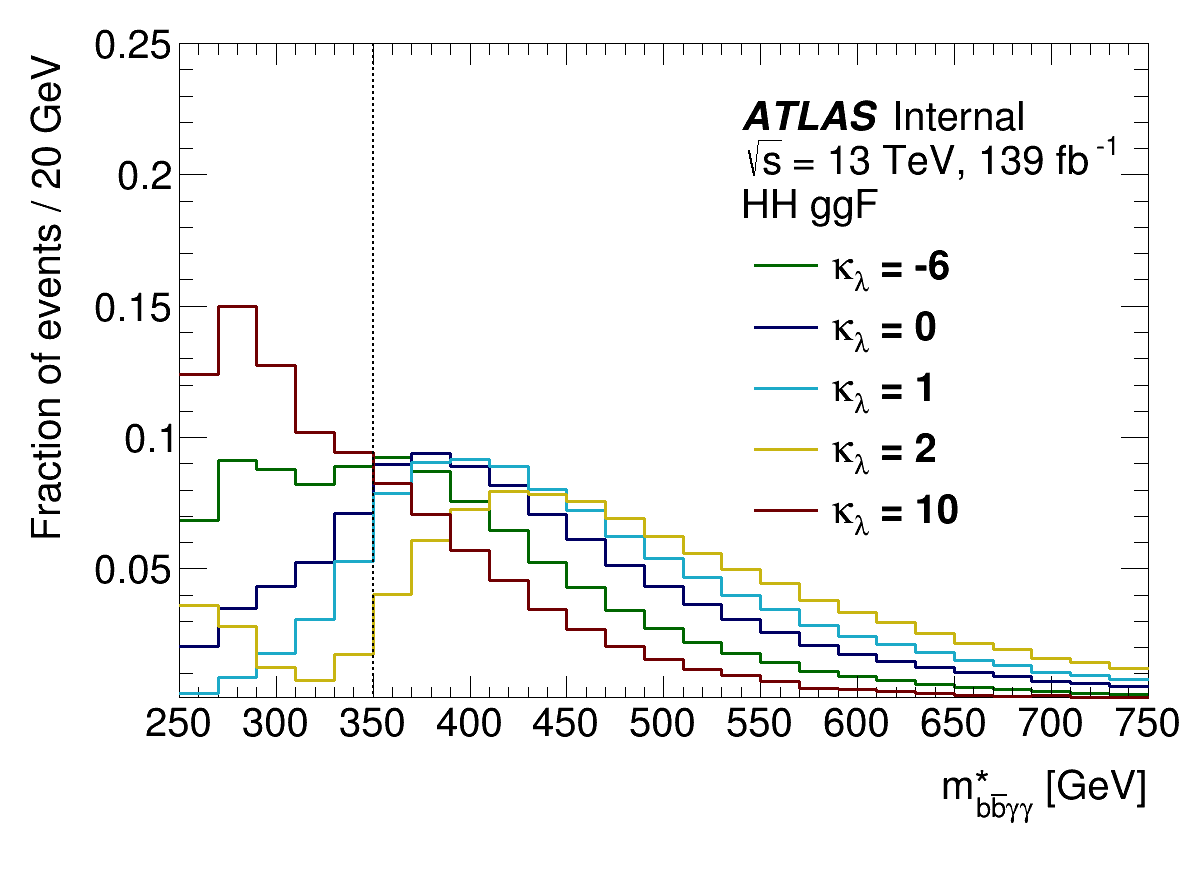
\includegraphics[width=.45\textwidth]{Ch5/Img/yybbstar_ggF.png} }
	\subfloat[VBF HH production mode][VBF HH production mode]{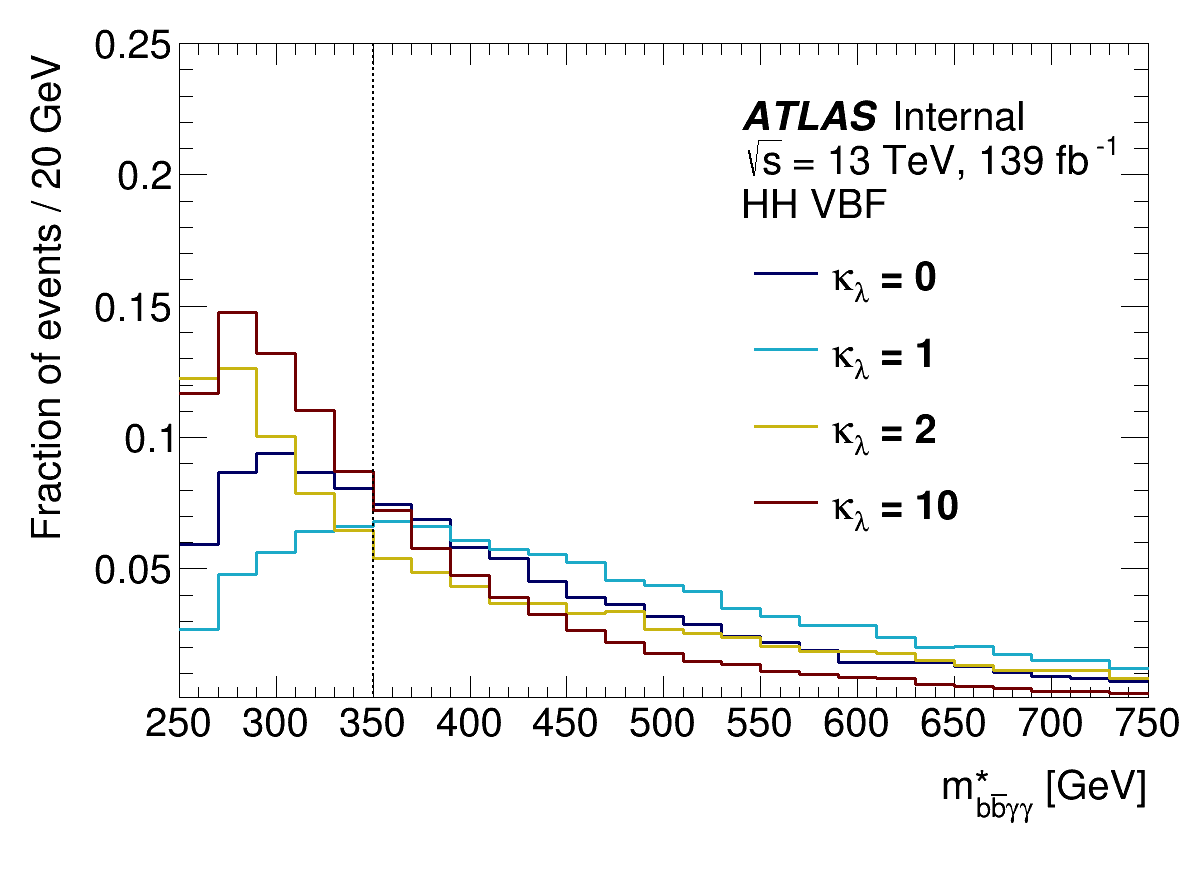
\includegraphics[width=.45\textwidth]{Ch5/Img/yybbstar_VBF.png}} 
    \caption{The $m_{b\bar{b}\gamma\gamma}^*$ distributions for non-resonant ggF HH (a) and VBF HH (b) signals with several \kl values. $m_{b\bar{b}\gamma\gamma}^* = $ 350 GeV is chosen as the separating boundary between categories targeting the SM and BSM \kl signals.}
    \label{fig:HHyybb:ObjEvt:Evt:myybb}
\end{figure}

In each mass region, a separate BDT is trained using \cite{XGBoost} to categorize ggF HH signal against a combination of the dominant MC backgrounds (continuum, $t\bar{t}H$, ggH and ZH). In the high-mass region, the \kl= 1 sample is used as signal while in the region targeting BSM scenarios (low-mass) the \kl= 10 sample is used as signal. Table \ref{tab:HHyybb:ObjEvt:Evt:BDT} lists the BDT inputs variables, the inputs set are use for both low and high-mass regions.

\begin{table}[ht]
    \centering
    \begin{tabular}{cc}
       \hline \hline
        Variable & Definition \\
        \hline \hline 
        $p_T$/\myy &  \pT of the two photons scaled by their invariant mass \myy. \\
        $\eta$ and $\phi$ & Pseudo-rapidity and azimuthal angle of the two photons. \\
        \hline 
        $b$-tagging score &  $b$-tagging score of the two jets.\\
        $\eta$, $\phi$ and \pT & \pT, pseudo-rapidity and azimuthal angle of the two jets. \\ 
        $m_{b\bar{b}}$ & $H\to b\bar{b}$ invariant mass. \\
        $H_T$ & Scalar sum of the \pT of the jets in the event. \\
        $\chi_{Wt}$ & single topness defined in Equation \ref{eq:HHyybb:ObjEvt:Evt:Topness}. \\
        \hline
        $E^{miss}_{T}$ and $\phi$ & Missing transverse momentum and its azimuthal angle. \\
        \hline\hline
    \end{tabular}
    \caption{Variables used in the BDT.}
    \label{tab:HHyybb:ObjEvt:Evt:BDT}
\end{table}
The single topness is defined as : 
\begin{equation}
    \chi_{W t}=\min \sqrt{\left(\frac{m_{j_{1} j_{2}}-m_{W}}{m_{W}}\right)^{2}+\left(\frac{m_{j_{1} j_{2} j_{3}}-m_{t}}{m_{t}}\right)^{2}},
    \label{eq:HHyybb:ObjEvt:Evt:Topness}
\end{equation}

where $m_W = $ 80 GeV, $m_t = $ 173 GeV, and the minimum is taken overall possible combinations of 3 jets in the event. No requirement on the $b$-tagging is applied for the $j_3$. \\

The BDT discriminate variable for low mass and high mass categories are shown in Figure \ref{fig:HHyybb:ObjEvt:Evt:dBDT}. In each mass region, two categories are defined based on the BDT score resulting in total of 4 categories as listed in Table \ref{tab:HHyybb:ObjEvt:Evt:Cat}.

\begin{figure}[ht]
    \centering
	\subfloat[Low mass region][Low mass region]{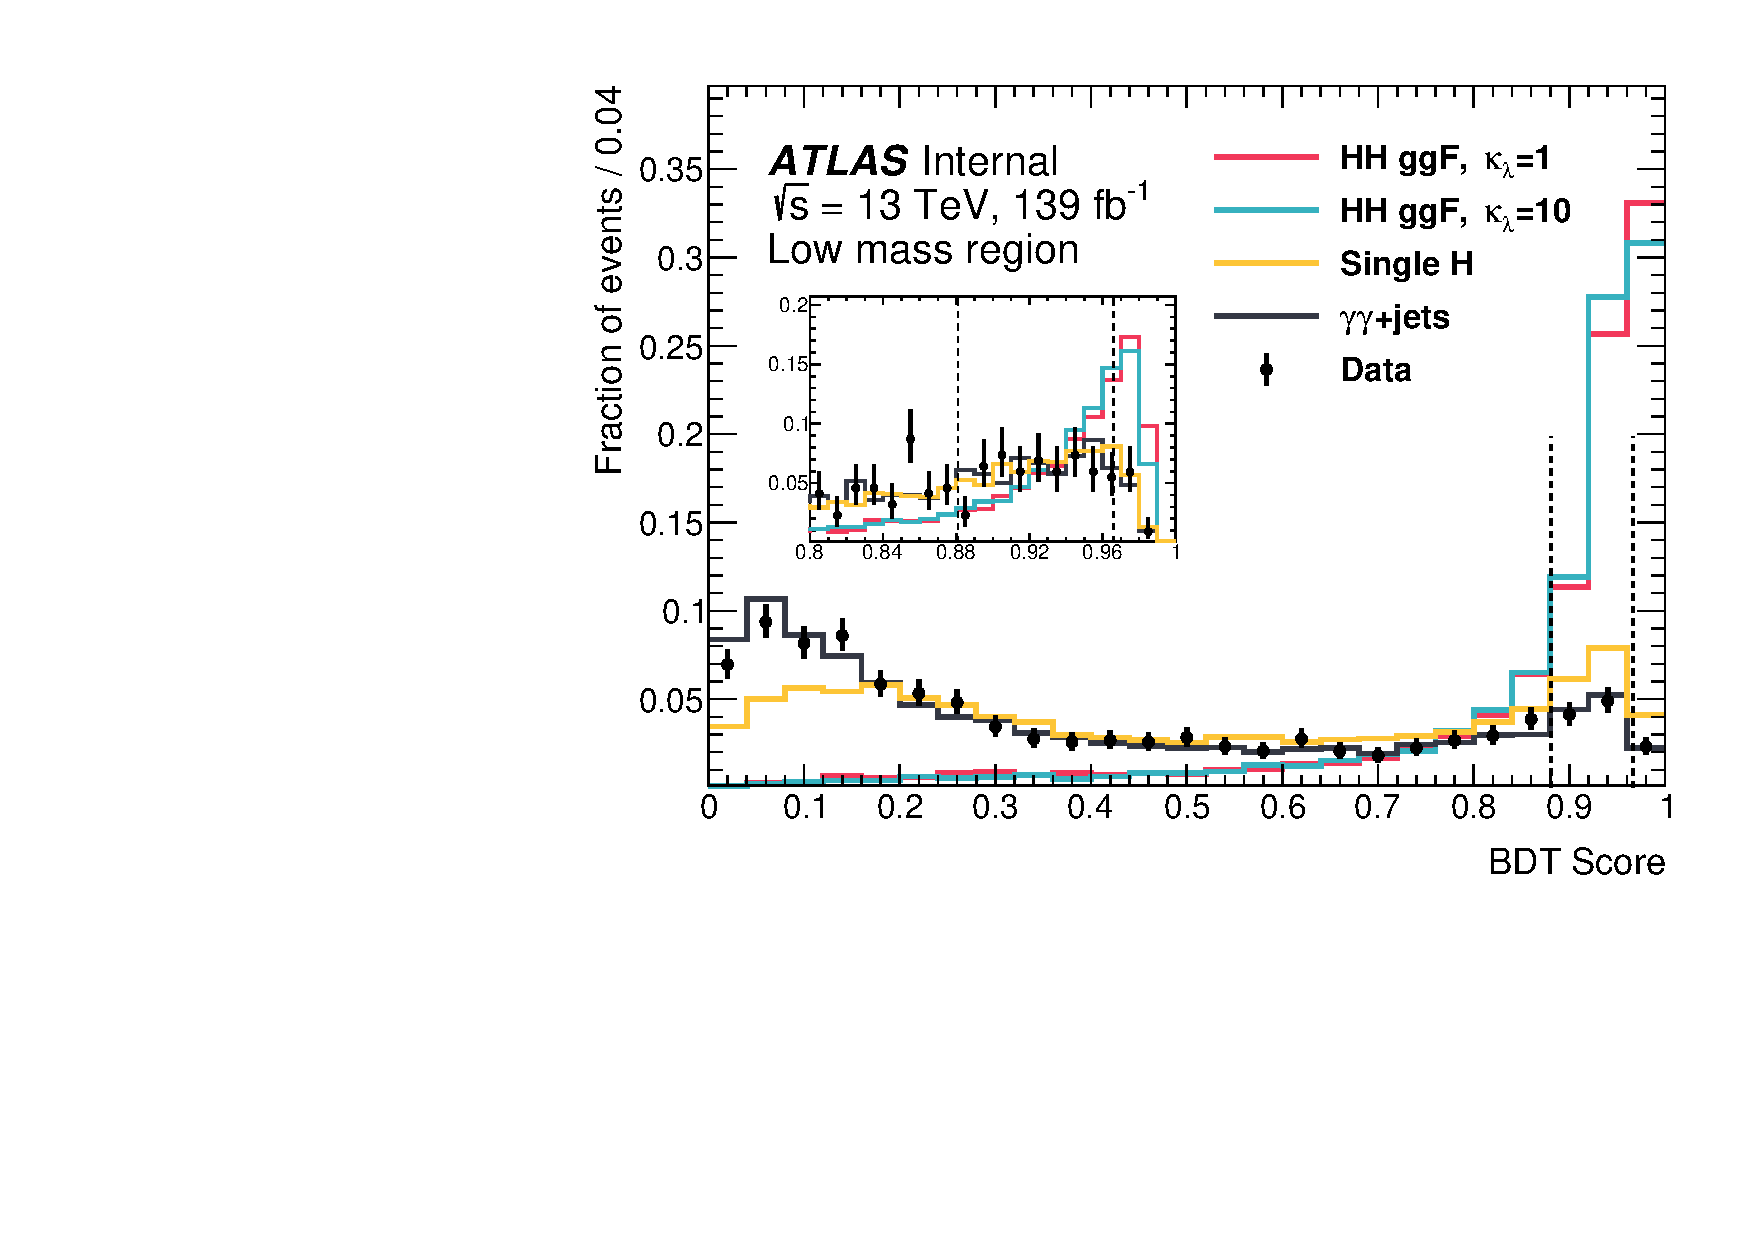
\includegraphics[width=.45\textwidth]{Ch5/Img/BDT_lowMass_Score.pdf} }
	\subfloat[High mass region][High mass region]{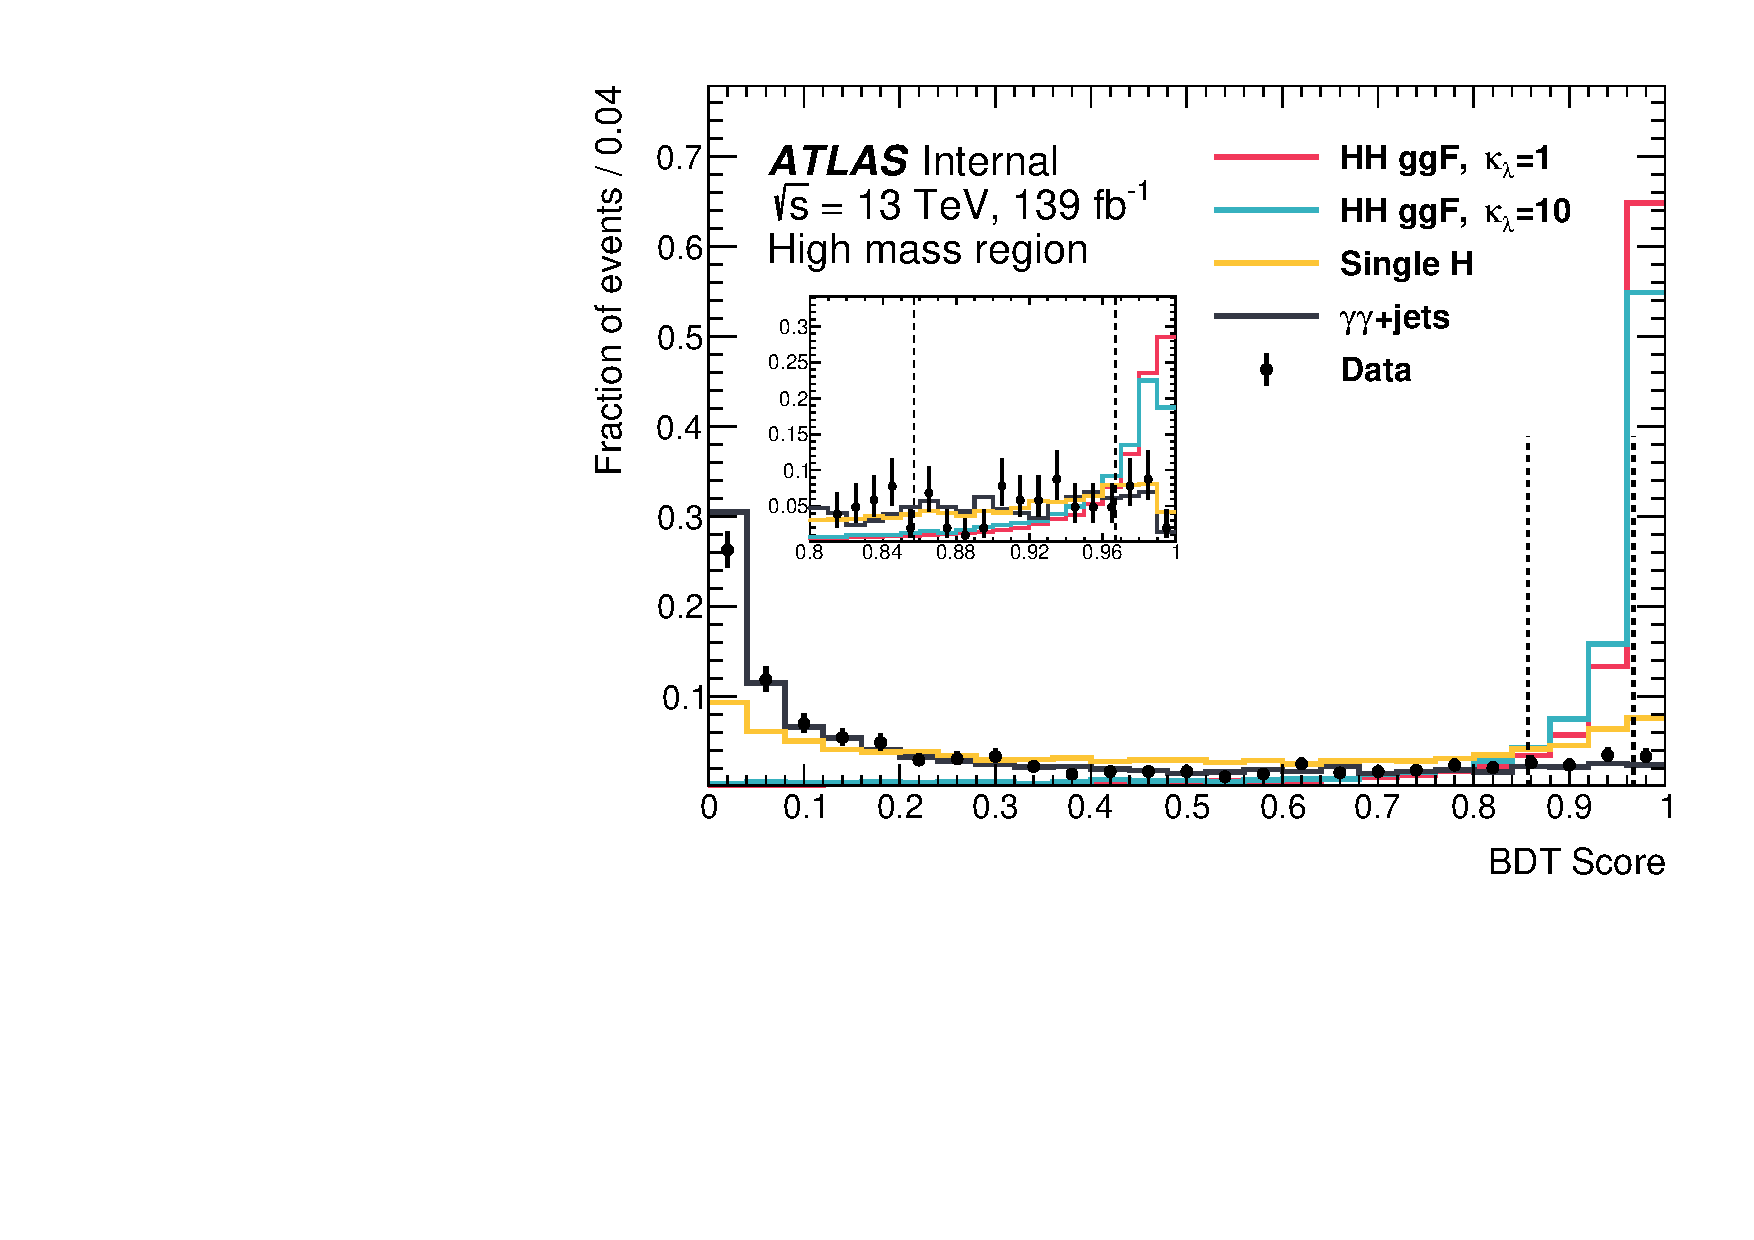
\includegraphics[width=.45\textwidth]{Ch5/Img/BDT_highMass_Score.pdf}} 
    \caption{The BDT score for the benchmark signals and the main backgrounds in the low- (a) and high- (b) mass region. Distributions are normalized to unit area. The dotted lines denote the category boundaries. Events with BDT score below 0.881 in the low mass region or below 0.857 in the high mass region are discarded.}
    \label{fig:HHyybb:ObjEvt:Evt:dBDT}
\end{figure}

\begin{table}[ht]
    \centering
    \begin{tabular}{cc}
    \hline\hline
        Category & Selection criteria \\
    \hline
    High mass BDT tight & $m_{b \bar{b} \gamma \gamma}^{*} \geq$ 350 GeV, BDT score $\in$ [0.967, 1] \\
    High mass BDT loose & $m_{b \bar{b} \gamma \gamma}^{*} \geq$ 350 GeV, BDT score $\in$ [0.857, 0.967] \\
    Low mass BDT tight & $m_{b \bar{b} \gamma \gamma}^{*} <$ 350 GeV, BDT score $\in$ [0.966, 1] \\
    Low mass BDT loose & $m_{b \bar{b} \gamma \gamma}^{*} <$ 350 GeV, BDT score $\in$ [0.881, 0.966] \\
     \hline\hline
    \end{tabular}
    \caption{Definition of the analysis categories.}
    \label{tab:HHyybb:ObjEvt:Evt:Cat}
\end{table}
The BDT approach improve the analysis significance by approximately 20\% compared to the previous cut-based selection used in the 36\ifb analysis \cite{yybb_36ifb}.  

\subsection{Event selection using Deep Neural Network}
\label{HHyybb:ObjEvt:DNN}

Following the same BDT strategy, a potential gain can be achieved using the Deep Neural Network (DNN). A separate DNN classifier is trained in each mass region using the same signal and backgrounds as the BDT. The DNNs attempt to classify each component against the rest (e.g continuum against signal + other backgrounds) in contrary to the BDT which only classify the signal against all background. \\
The architecture of the two classifiers is identical. The classifiers are built using the \textsc{Keras} library with \textsc{TensorFlow} as backend \cite{keras,tensorflow}. it Contains an input layer constructed form a batch normalization and a fully connected layer, then five fully connected hidden layers with each one is flowed with a dropout layer, and finally an output layer. Each of the fully connected layers has 128 nodes activated using Rectified Linear Unit (ReLU) activation function, and their weights are randomly initialized by sampling from a truncated distribution centered on zero with width given by $\sqrt{\frac{2}{N_{inputs}}}$ where $N_{inputs}$ is the number of input features. The dropout layers are used to improve the robustness of the training and reduce overfitting effects, for high mass region model the dropout rate is 11\%, while for low mass region, the dropout rate is 22.5\%. The batch normalization layer is used standardizes the inputs to the first layer. The output layer is 4-nodes wide and activated using softmax activation function which allows one to interpret the outputs as the probability for each associated class (ggF HH, ZH, ttH or continuum) given the input event. During the training, a weighted categorical cross-entropy is used as loss function and Adam optimizer for network weight optimization.\\
Weights of the loss function correspond to the event class weight computed as the weight of event j associated to class i as :
\begin{equation}
    weight_i^j = \frac{\sum_{j,i} N_i^j}{n\times\sum_{j} N_i^j},
\end{equation}
where $n=\sum i = 4$ is number of classes, $\sum_{j,i} N_i^j$ is the total number of events a cross all classes and $\sum_{j} N_i^j$ is the total number of events in the given class i. The event class weight allows the models to perform similarly between classes and reduces the unbalanced issue in data which affects the model classification ability.\\
The two DNN models are trained with a learning rate of $1e^{-4}$ and a batch size fixed to 1000 events, with a maximum number of epochs set to 100. Similar to the CNN developed for photon identification, an early stopping metric evaluated on the validation data sample throughout the training is imposed during the training phase.\\ 
DNNs use almost the same inputs variables as the BDT list in Table \ref{tab:HHyybb:ObjEvt:Evt:BDT} except for the single topness, $H_T$, the missing transverse energy and its azimuthal angle which are not included. The class-invariant symmetries (detector symmetry) complexity is removed by rotating all events around the beam axis in such a way that the leading photon has $\phi=0$ . \\
Figure \ref{fig:HHyybb:ObjEvt:DNN:Loss} shows the evaluation of the loss function during the training time for the training and validation dataset, the early stopping stop the training around epoch 40 to avoid overfitting. The low mass model shows a high loss error compared to high mass one which translate the signal like background distribution, reducing the model separation in the low mass region.
\begin{figure}[ht]
    \centering
    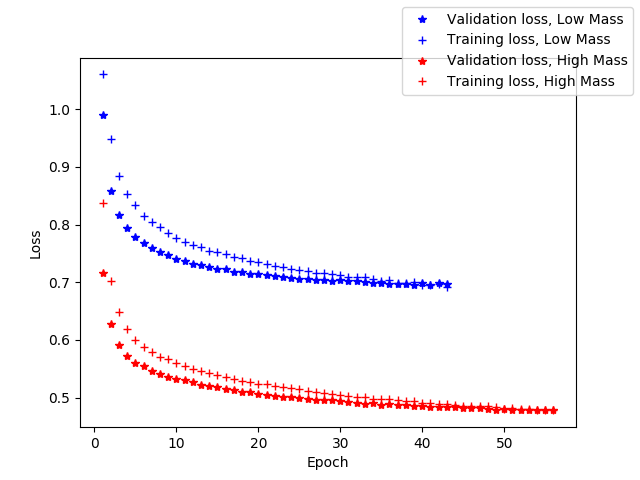
\includegraphics[width=0.6\textwidth]{Ch5/Img/Loss_DNN.png}
    \caption{Evaluation of the loss function for high mass (red) and low mass (blue) DNNs as a function of epoch number.}
    \label{fig:HHyybb:ObjEvt:DNN:Loss}
\end{figure}
One of the performance measurement of an classifier is the confusion matrix, the matrix compares the actual target values with those predicted by the model. This gives a holistic view of the performance of the classification model as well as the associated errors. Figure \ref{fig:HHyybb:ObjEvt:DNN:CM} shows the confusion matrix for high mass and low mass models. Note that the threshold value for the prediction of the model set to 0.5 on the softmax outputs. Both models show a high ($\sim$19\%) confusion between the ggF HH signal and the ZH background coming from the similarity between the event topology of the two processes. Similar for ttH event are almost confused with continuum or ZH. At low mass region, the performance clearly decreases due to the similarity in the kinematics and events topology between ggF HH and backgrounds.
\begin{figure}[ht]
    \centering
    \subfloat[][]{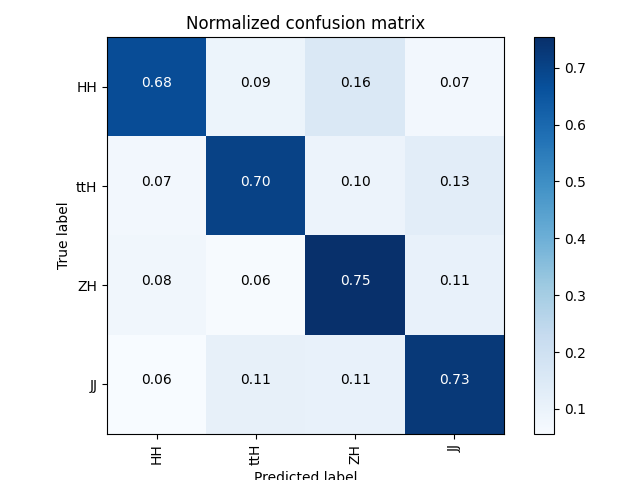
\includegraphics[width=.5\textwidth]{Ch5/Img/cm_SM.png}}
    \subfloat[][]{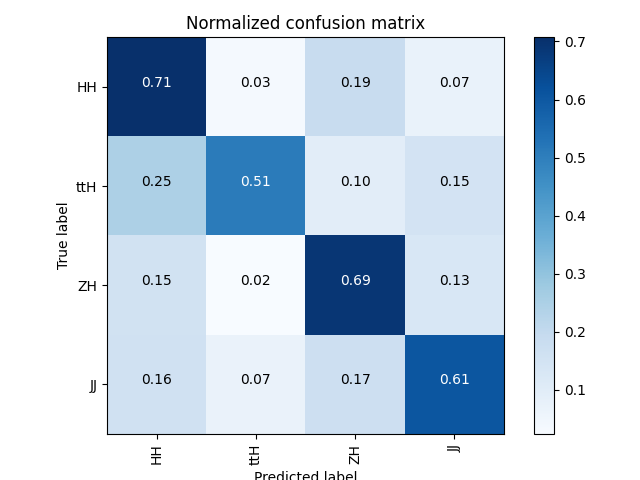
\includegraphics[width=.5\textwidth]{Ch5/Img/cm_BSM.png}}
    \caption{Normalized (to unity) confusion matrix for (a) high mass and (b) low mass models. JJ here denote the continuum $\gamma\gamma+$jets.}
    \label{fig:HHyybb:ObjEvt:DNN:CM}
\end{figure}

\subsubsection{Discriminant variable}
The four outputs of the softmax layer are combined in a single discriminant denoted $d_{HH}$ for each region, the probabilities are normalized to the corresponding process cross section.
\begin{equation}
    d_{HH}^{HM} = log \left(\frac{\sigma_{SM}.p_{HH}}{\sigma_{ZH}.p_{ZH}+\sigma_{ttH}.p_{ttH}+\sigma_{\gamma\gamma+jets}.p_{\gamma\gamma+jets}}\right)
    \label{eq:DHH_HM}
\end{equation}
\begin{equation}
    d_{HH}^{LM} = log \left(\frac{\sigma_{\kappa_\lambda10}.p_{HH}}{\sigma_{ZH}.p_{ZH}+\sigma_{ttH}.p_{ttH}+\sigma_{\gamma\gamma+jets}.p_{\gamma\gamma+jets}}\right)
    \label{eq:DHH_LM}
\end{equation}
$d_{HH}^{HM}$ in Equation \ref{eq:DHH_HM} represents the $d_{HH}$ discriminant for high mass region, while Equation \ref{eq:DHH_LM} is the $d_{HH}$ discriminant in low mass region. \\

Figure \ref{fig:HHyybb:ObjEvt:DNN:dHH} shows the distribution of $d_{HH}$ discriminant for each process (ggF HH, ZH, ttH and continuum) in each mass region. At high mass $d_{HH}$ shows a clear separation between the HH and other process, while for low mass the discrepancy is low as expected. The side-band data flows the continuum background perfectly indicting a good modelling of the $d_{HH}$ distribution. 
\begin{figure}[ht]
    \centering
    \subfloat[][]{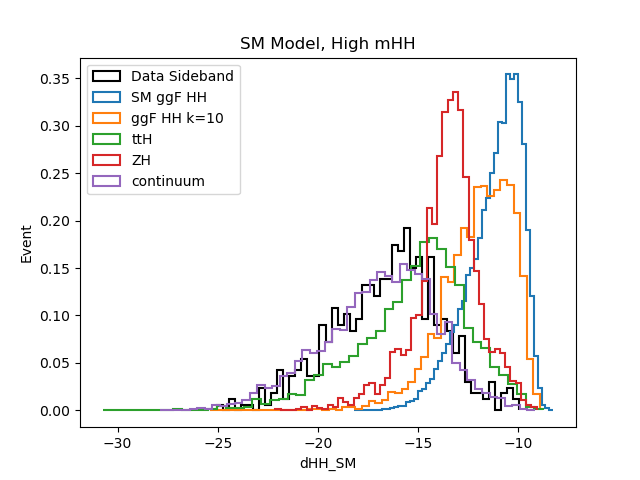
\includegraphics[width=.5\textwidth]{Ch5/Img/dHH_SM.png}}
    \subfloat[][]{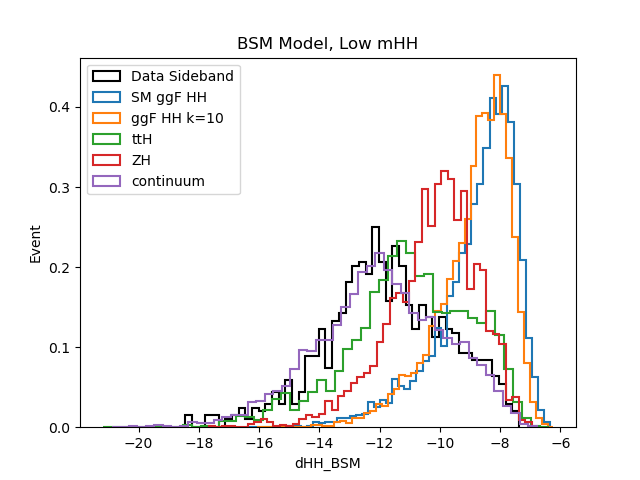
\includegraphics[width=.5\textwidth]{Ch5/Img/dHH_BSM.png}}
    \caption{$d_{HH}$ discriminant distribution in (a) high mass and (b) low mass. The black line shows the real data in the side band region ($m_{\gamma\gamma}\in[105,120] \cup [130,160]$).}
    \label{fig:HHyybb:ObjEvt:DNN:dHH}
\end{figure}

\subsubsection{Significance scan}
In each region the corresponding discriminant is scanned in $90<m_{bb}<140$ GeV area to define two orthogonal categories high $d_{HH}$ and low $d_{HH}$ with a maximum significance, the category with highest significance has at least 0.8 continuum events in the $123<m_{\gamma\gamma}<127$ GeV region which corresponds to 9 background events in the $m_{\gamma\gamma}\in[105,120] \cup [130,160]$ GeV sufficient to perform an \myy fit, this is done in a similar way to the BDT. The significance is computed using the Asimov formula \cite{Z} defined as : 
\begin{equation}
    Z = \sqrt{2\left[(s+b)\times log(1+s/b)-s\right]},
\end{equation}

where, s is the HH signal yield and b is the total background yield. In total 4 categories are defined, two for low mass region and two in high mass region. Significance of the 4 categories are then combined for the final significance. Table \ref{tab:Sig} lists the significance in each category.
\begin{table}[ht]
    \centering
    \begin{tabular}{ccc}
        \hline\hline
        Categories & SM ggF HH & BSM $\kappa_\lambda$=10 ggF HH \\
        High Mass, High $d_{HH}$ & 0.53 & 2.45 \\
        High Mass, Low $d_{HH}$ & 0.11 & 0.94 \\
        Low Mass, High $d_{HH}$ & 0.03 & 2.21 \\
        Low Mass, Low $d_{HH}$ & 0.01 & 0.54 \\
        \hline
        Combined & 0.54$\sigma$ & 3.47$\sigma$ \\
        \hline
        \hline
    \end{tabular}
    \caption{Significance in each categories for SM HH and BSM $\kappa_\lambda$=10 signal.}
    \label{tab:Sig}
\end{table}
The proposed selection based on a DNN shows similar performances with respect to the BDT with less inputs variables. The removed variables in the DNN have a high importance in the BDT case, thus including those variables in the DNN for the Run-3 analysis will enhance the DNN performance. The BDT event categorization is used a baseline for Run-2 \HHyybb analysis since it shows a robustness and good improvement, while the DNN based selection is kept for next analysis rounds (Run-3). \\

The \myy distribution in each of the BDT category is shown in Figure \ref{fig:HHyybb:ObjEvt:myy}. The background decomposition is described in Section \ref{HHyybb:Modelling:Bkg}.

\begin{figure}[ht]
    \centering
    \subfloat[][High mass, BDT tight]{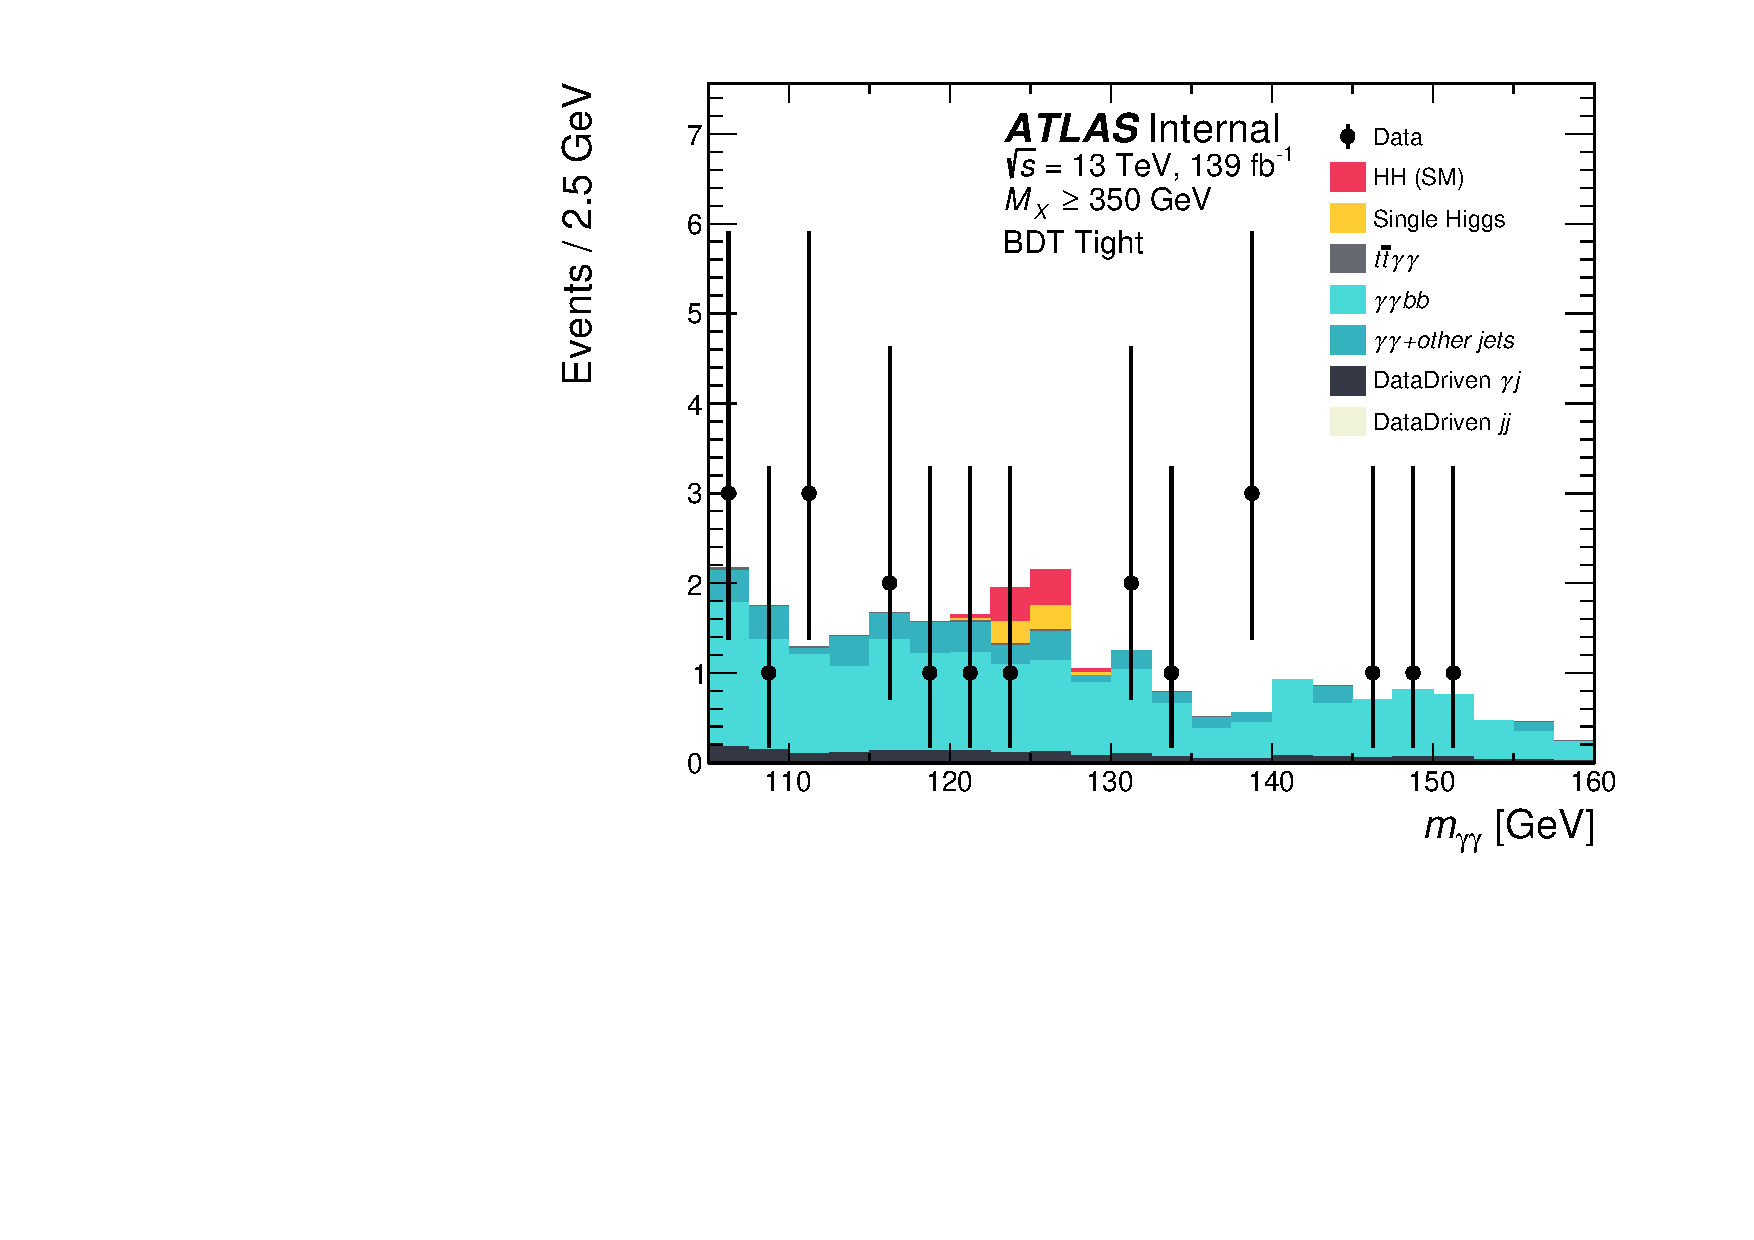
\includegraphics[width=.5\textwidth]{Ch5/Img/m_yy_XGBoost_btag77_withTop_BCal_tightScore_HMass.pdf}}
    \subfloat[][Low mass, BDT tight ]{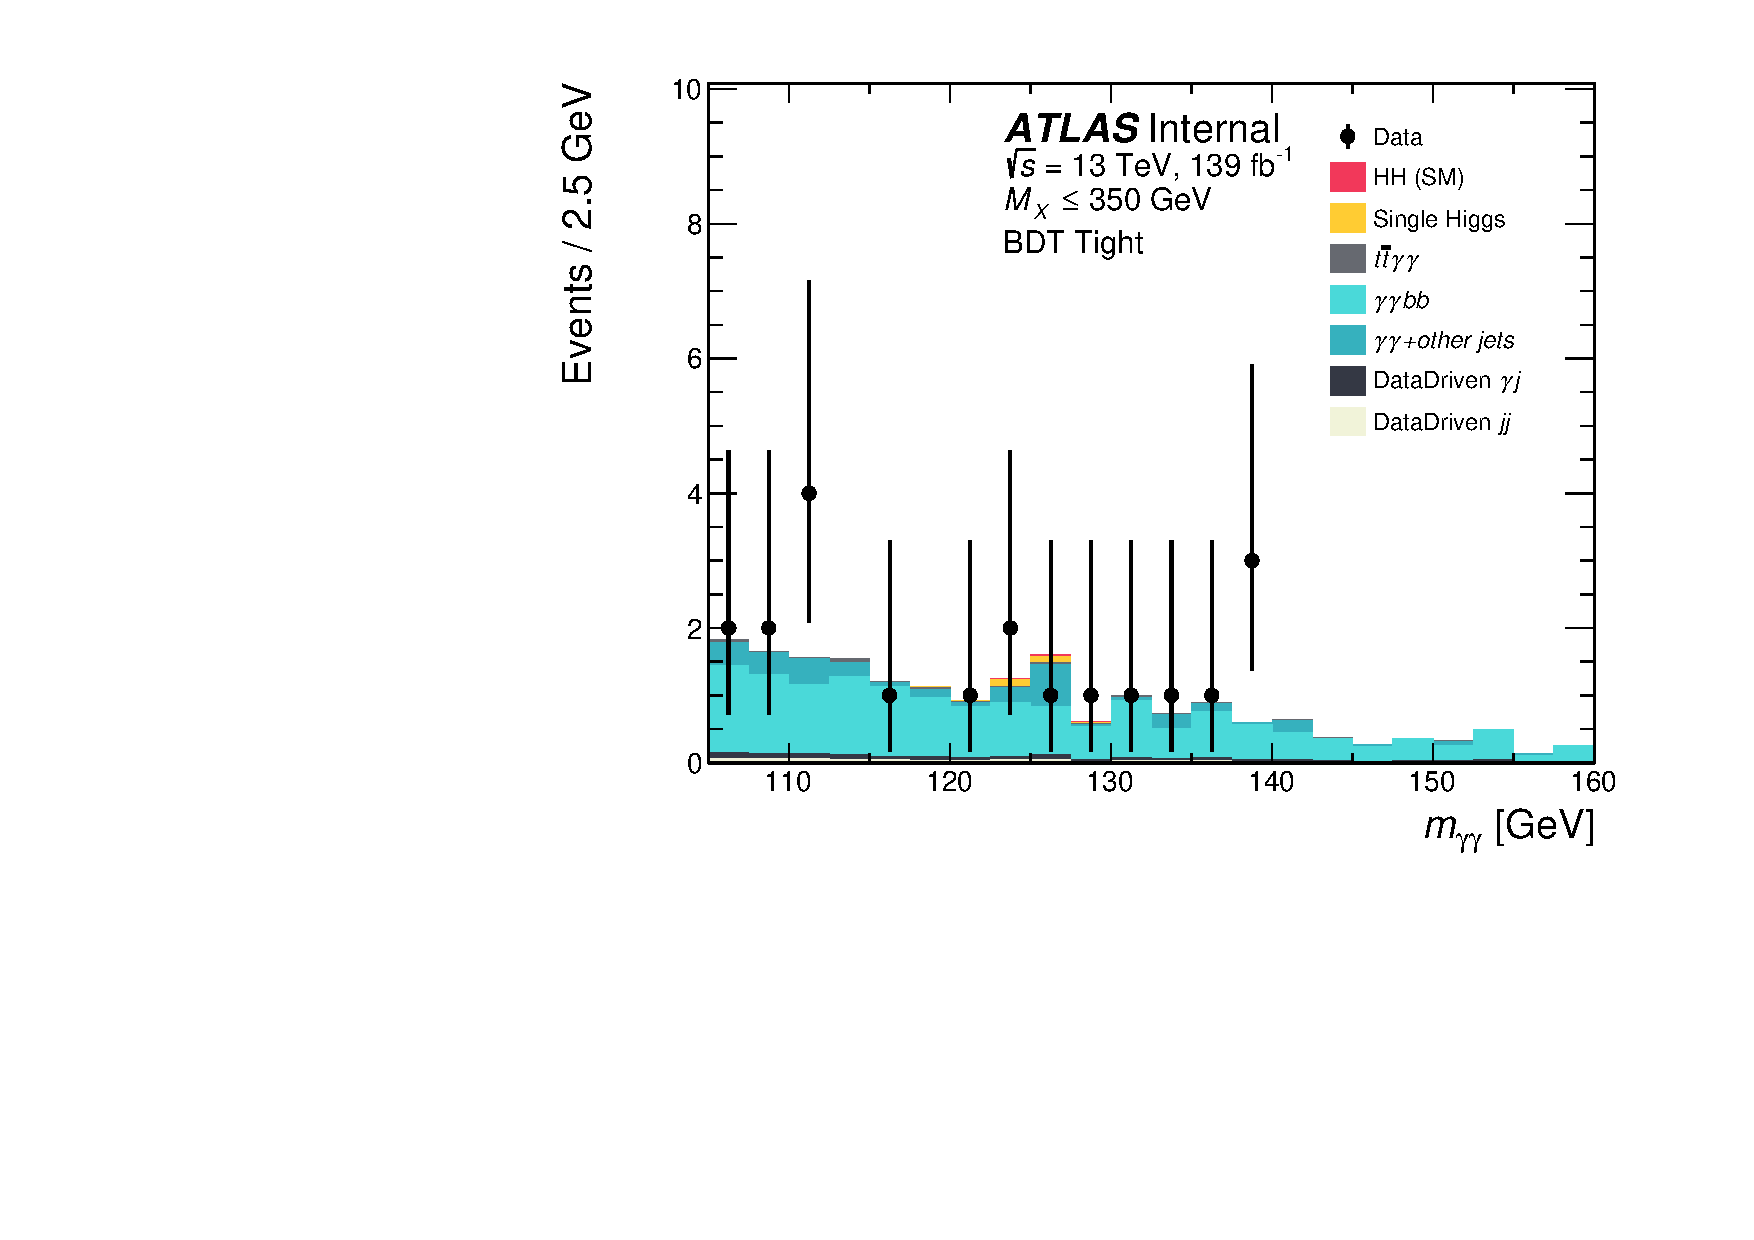
\includegraphics[width=.5\textwidth]{Ch5/Img/m_yy_XGBoost_btag77_withTop_BCal_tightScore_LMass.pdf}} \\
    \subfloat[][High mass, BDT loose]{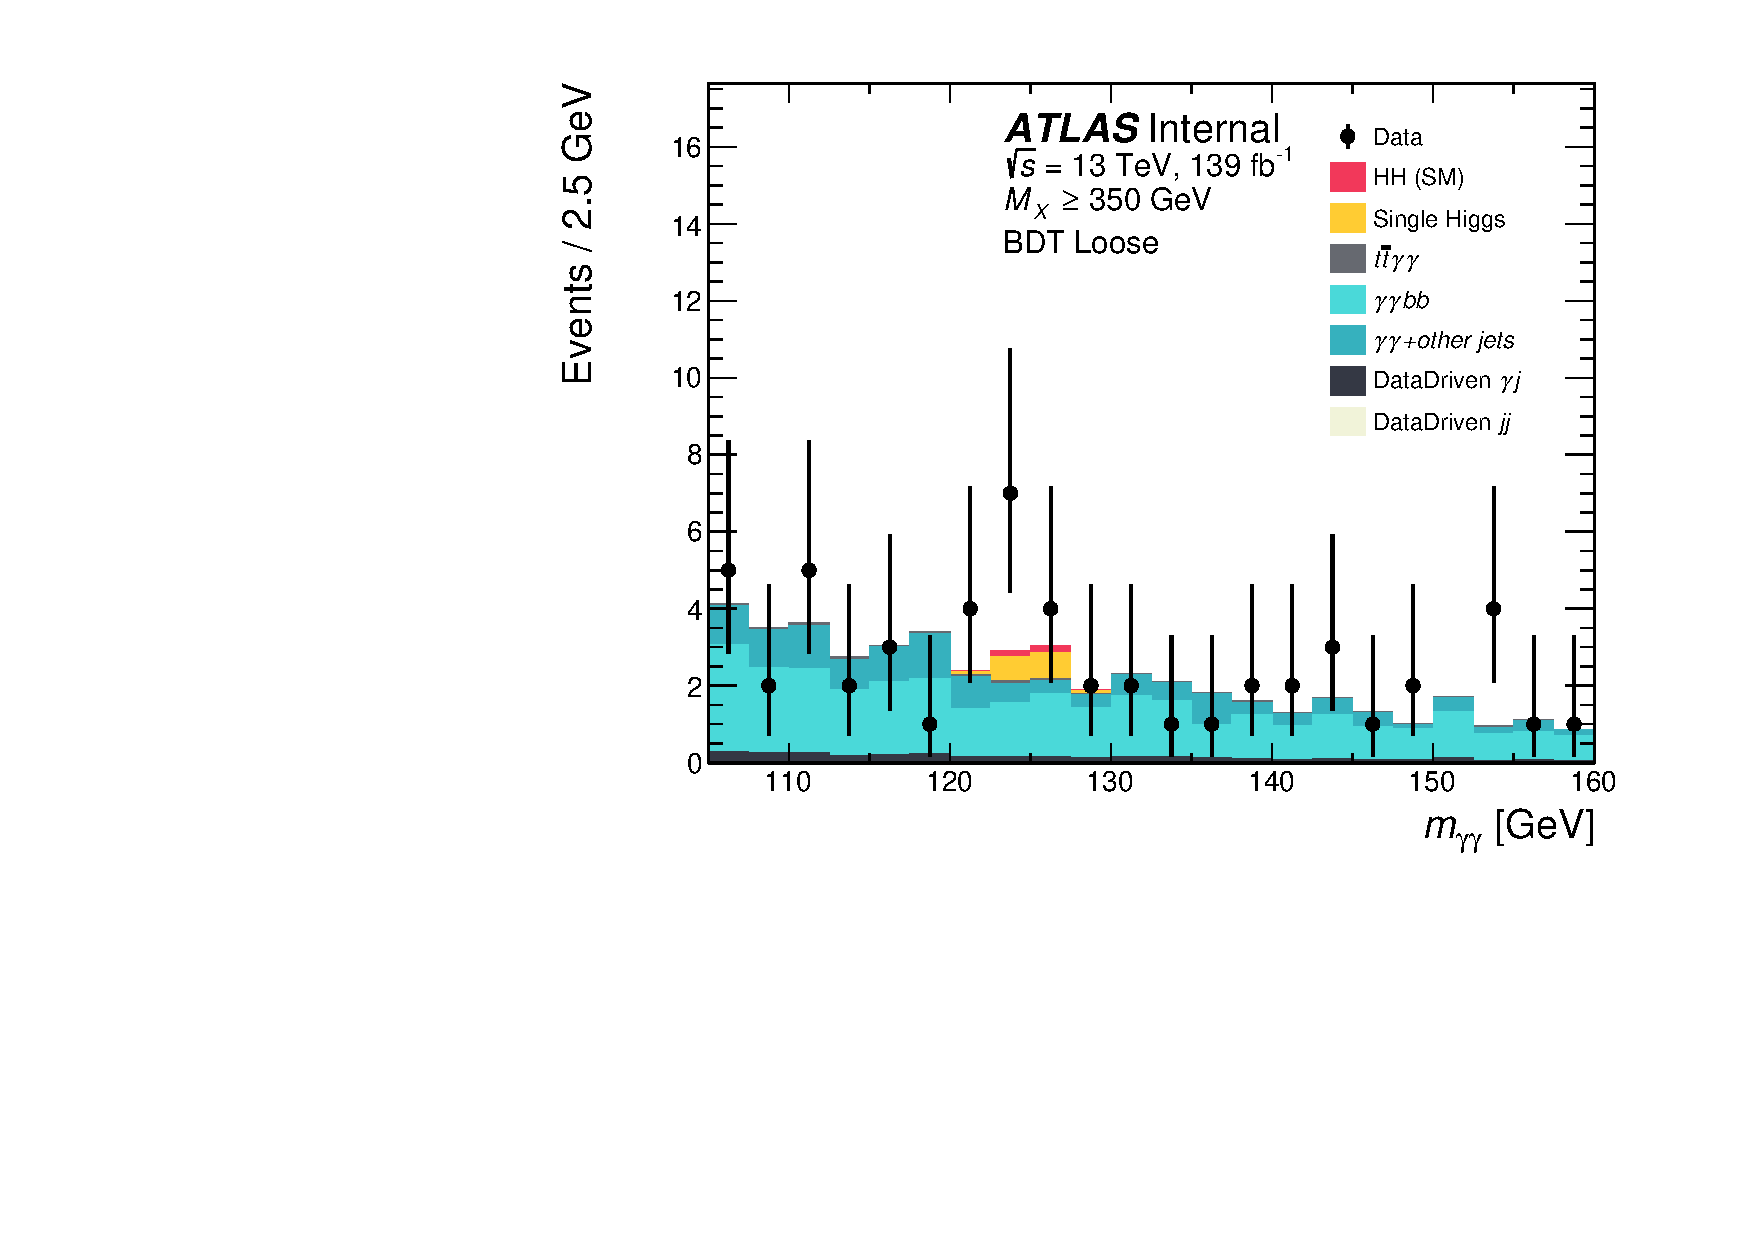
\includegraphics[width=.5\textwidth]{Ch5/Img/m_yy_XGBoost_btag77_withTop_BCal_looseScore_HMass.pdf}}
    \subfloat[][Low mass, BDT loose ]{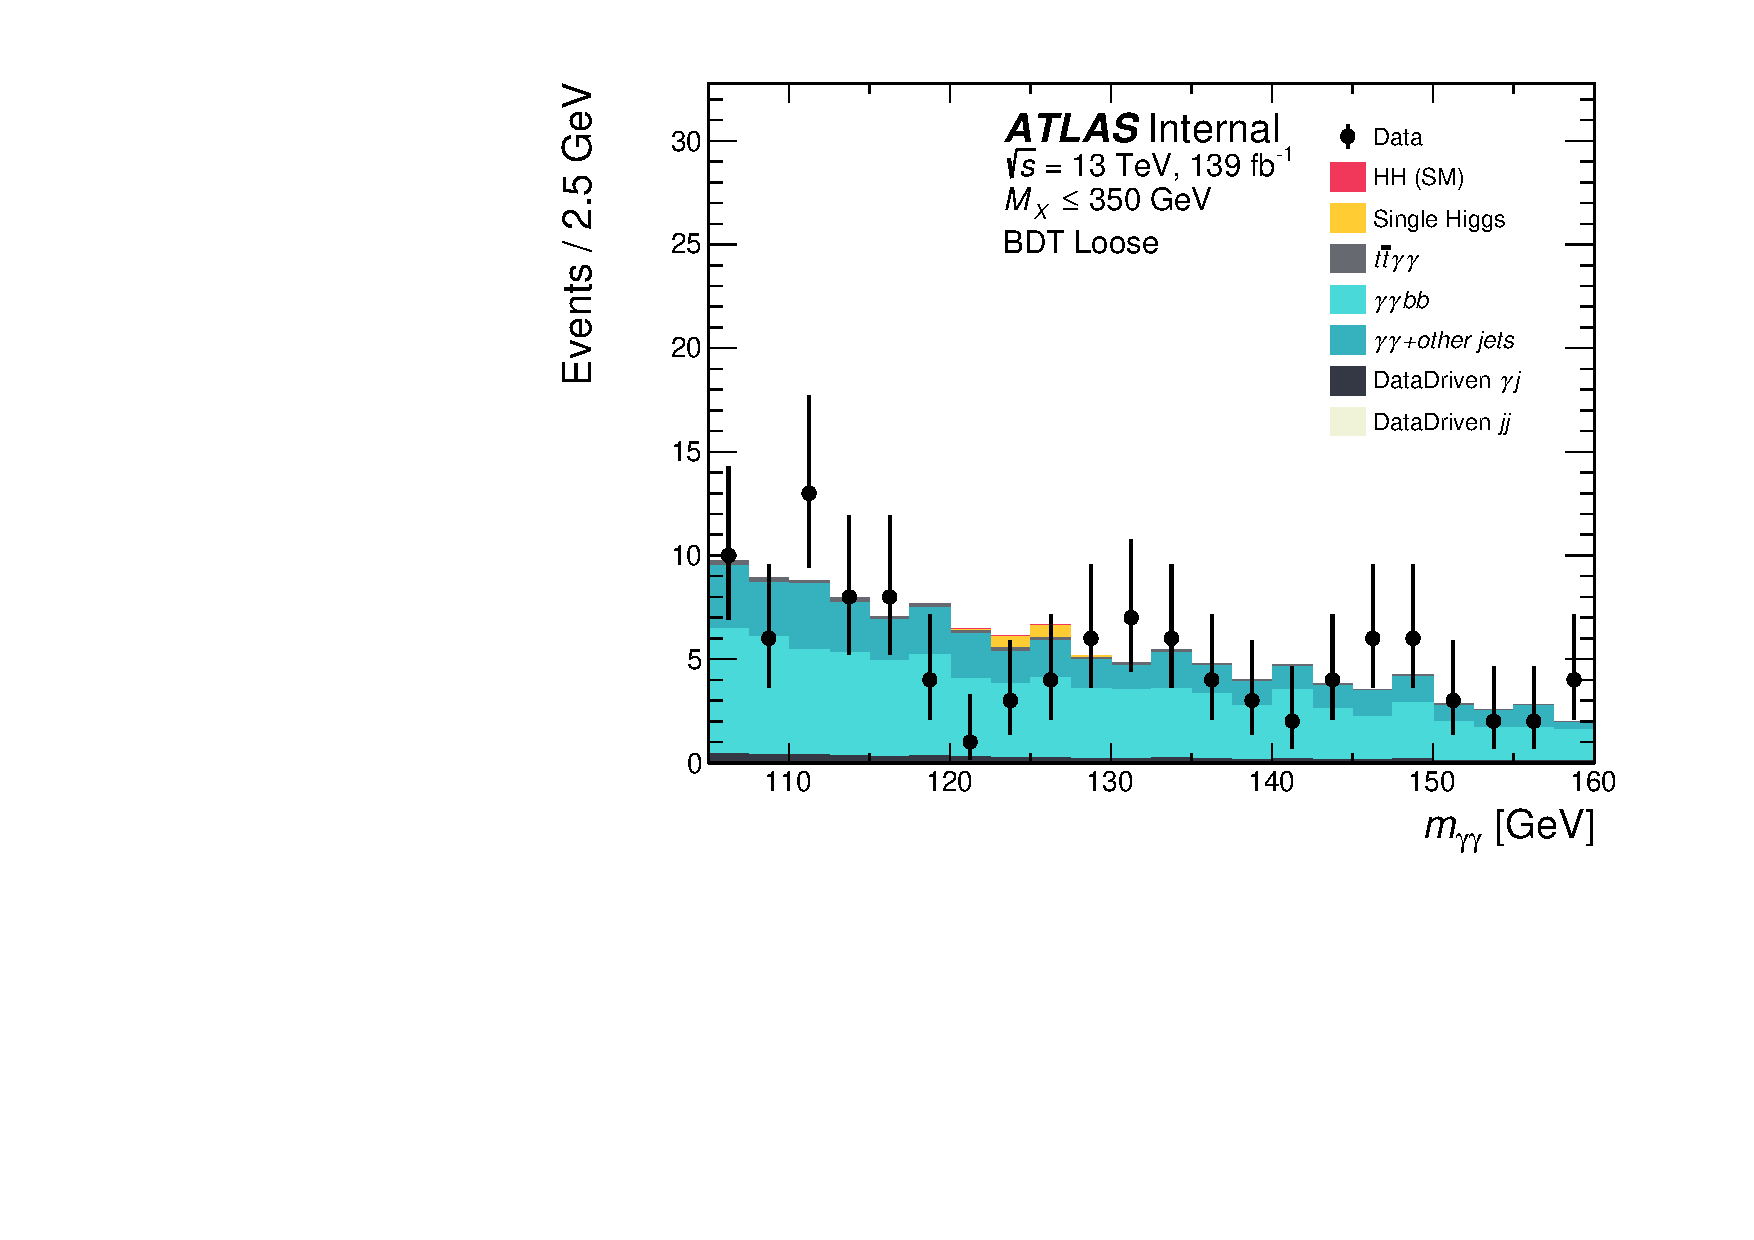
\includegraphics[width=.5\textwidth]{Ch5/Img/m_yy_XGBoost_btag77_withTop_BCal_looseScore_LMass.pdf}}
  
    \caption{Distributions of \myy in all signal categories. The continuum background is scaled by the $\gamma\gamma$, $\gamma$-jets or jet-$\gamma$, and jet-jet fractions and normalized to the data side-band.}
    \label{fig:HHyybb:ObjEvt:myy}
\end{figure}



\section{Signal and background modelling}
\label{HHyybb:Modelling}

To extract the \HHyybb signal yield, a fit to the \myy in the range 150 $<$ \myy $<$ 160 GeV. Analytic functions are used to describe the signal, single Higgs background and the continuum background. Parameters of the signal and the peaking single Higgs backgrounds shapes are fixed on MC distributions, while the background parameters are directly constrained on the data.   

\subsection{Signal and single Higgs parameterization}
\label{HHyybb:Modelling:Sig}

Both signal and peaking single Higgs backgrounds can be described analytically by a double-sided Crystal Ball (DSCB) function which is characterized by a Gaussian core and asymmetric power law tails \cite{Higgs_2018}, defined as :

\begin{equation}
    f_{\mathrm{DSCB}}\left(m_{\gamma \gamma}\right)=N \times\left\{\begin{array}{ll}
e^{-t^{2} / 2} &  if \ -\alpha_{low } \leq t \leq \alpha_{high } \\

\frac{e^{-\frac{1}{2} \alpha_{low }^{2}}} {  \left[  \frac{1}{ R_{low} } \left(R_{low }-\alpha_{low }-t\right) \right]^{n_{low }}} & if \ t<-\alpha_{low } \\

\frac{e^{-\frac{1}{2} \alpha_{high }^{2}}} {  \left[  \frac{1}{ R_{high} } \left(R_{high }-\alpha_{high }-t\right) \right]^{n_{high }}} &  if \ t>\alpha_{high }
\end{array}\right.
\end{equation}
with $t = \frac{m_{\gamma\gamma} - \mu_{CB}}{\sigma_{CB}}$. $\mu_{CB}$ and $\sigma_{CB}$ describe the mean and the width of the Gaussian core, $\alpha_{low/high}$ describes the transition from the core to the tails of the distribution and $n_{low/high}$ describe the tails. N normalizes the distribution. The explicit separation of the Gaussian core from the tails in this function allows an easy treatment of the systematic uncertainties, as energy scale uncertainty allows a variation of the mean and the resolution systematic allows the variation of the width, thus the choice of this function.\\
The normalizations are obtained from the expected MC yields. For each category (BDT categories), the parameters of the DSCB are fixed from the fit of the \myy obtained from MC simulation of the ggF and VBF HH processes with \kl = 1, since no significance dependence of the functional form with \kl was found. Fitted parameters are further allowed to vary only within the systematic uncertainties on the energy scale and resolution. Injection tests are performed to quantify potential biases from the signal HH only fit and signal + single Higgs fit. No statistically significant biases ($<$ 10\%) were observed in both tests, thus the same parameterized functions are used to fit the signal and single Higgs backgrounds.    

\subsection{Continuum background parameterization}
\label{HHyybb:Modelling:Bkg}

The continuum background estimation is done in a data-driven way, MC used only to chose the functional form and its parameters are then left completely free in the fit to data, allowing to reduce uncertainties due to a background mismodelling. The background is decomposed to several component to take into account contribution from the continuous $\gamma\gamma$, $\gamma$j and jj fake photons components. The decomposition is done using a 2x2 ABCD side-band method \cite{ABCD}, in which an equation system is built and the equation system is solved to determine the relative contribution of each components (purity). The purities are measured inclusively and each BDT category. Inclusively the purity of the $\gamma\gamma$ events is around 85$\pm$2.9\% and the remaining 15$\pm$2.8\% consists of the $\gamma$+jet events and a negligible amount of the jj events. The $\gamma\gamma$ contribution increases after the BDT selection since a higher BDT score, the BDT tends to select events with higher photon \pT thus more real photons. The decomposition is shown in Figure \ref{fig:HHyybb:Modelling:Bkg:Decom}. 

\begin{figure}[ht]
    \centering
    \subfloat[][]{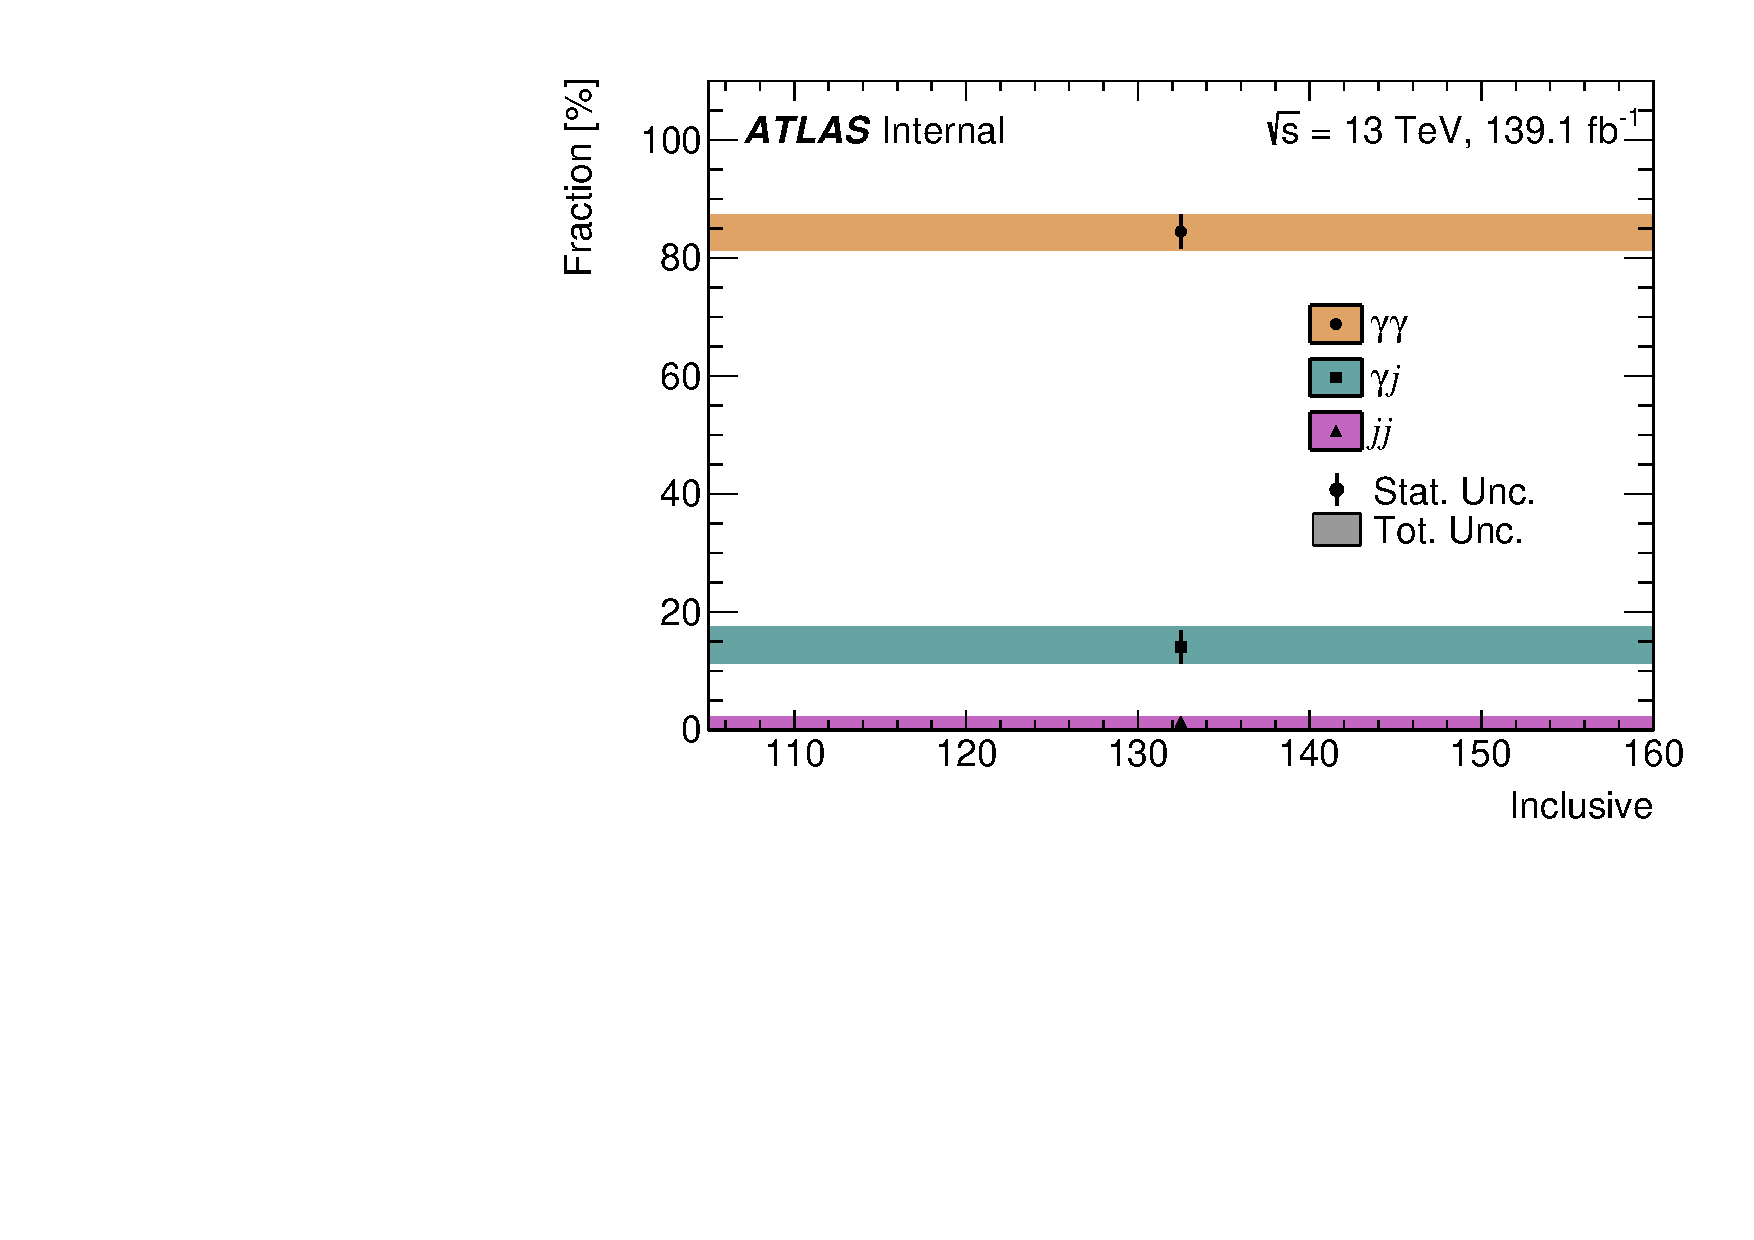
\includegraphics[width=.5\textwidth]{Ch5/Img/figures_BackgroundDecomposition_plot_purity_inclusive.pdf}}
    \subfloat[][]{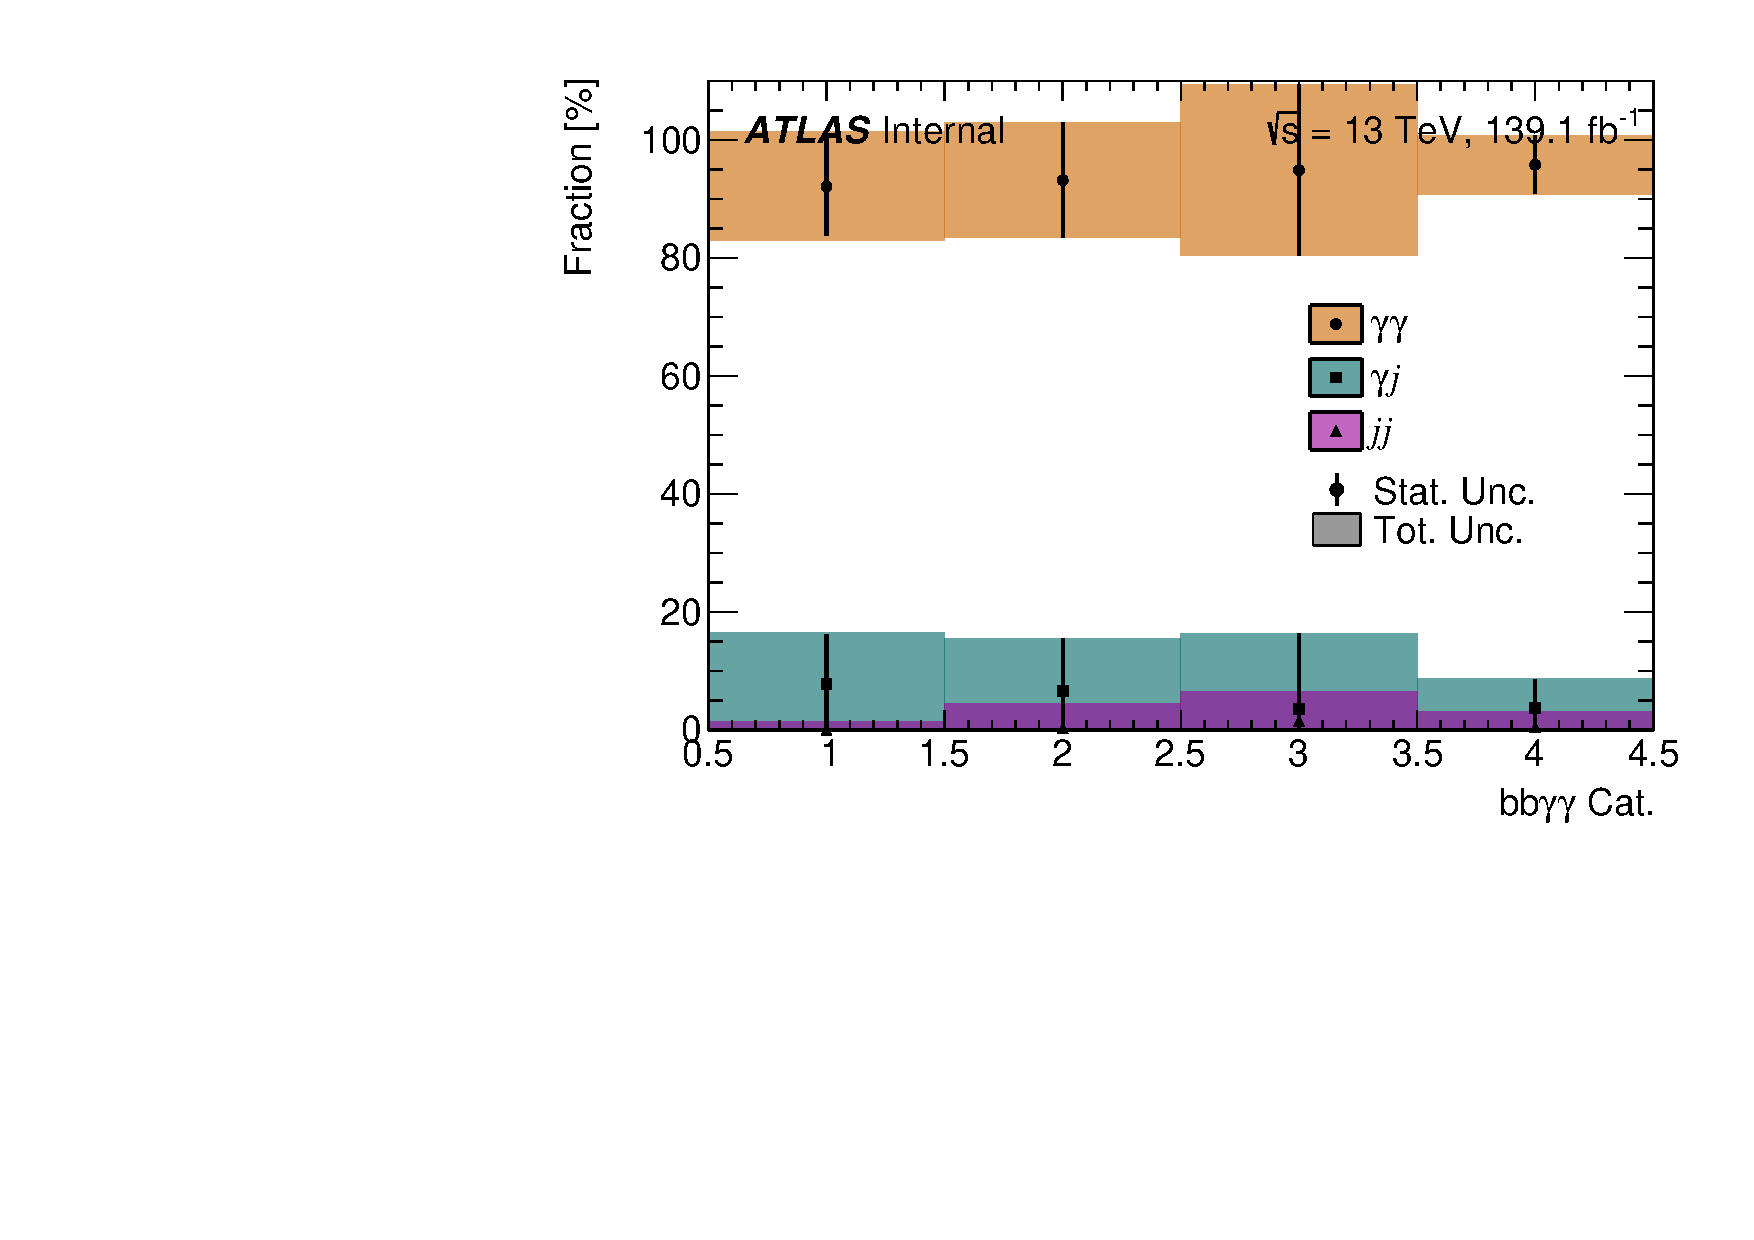
\includegraphics[width=.5\textwidth]{Ch5/Img/figures_BackgroundDecomposition_plot_purity_yybb_nonRes_XGBoost_btag77_BCal_Cat.pdf}}
    \caption{$\gamma\gamma$,$\gamma$j/$j\gamma$, and jet-jet fractions in the inclusive (a) and the BDT categories (b). In the BDT figure bin 1 corresponds to the High mass BDT tight category, bin 2 corresponds to the High mass BDT loose category, bin 3 corresponds to the Low mass BDT tight category, and finally bin 4 corresponds to the Low mass BDT loose category.}
    \label{fig:HHyybb:Modelling:Bkg:Decom}
\end{figure}

The functional form is chosen by fitting a MC background template. Given the high $\gamma\gamma$ purity, the template is constructed from the \texttt{SHERPA} $\gamma\gamma$+jets normalized to the data side-band. The bias on the specific choice of functional form (absorb potential signal or create an artificial signal) is determined by the spurious signal test. 

\subsubsection{Spurious signal test}
\label{HHyybb:Modelling:Bkg:SS}
The spurious signal (SS) refers to any potential fake signal $N_{SS}$ obtained from fitting the smooth background distribution to a function that describes the signal plus background shape. The $N_{SS}$ is taken to be the largest number of fitted signal events computed for Higgs masses varying in intervals of 1 GeV from 121 GeV to 129 GeV. The SS requires the tested function fulfill one of the following criteria: 
\begin{itemize}
    \item $N_{SS} < $ 10\% $N_{s}^{exp}$, where $N_{s}^{exp}$ is the expected number of signal events within the BDT category. 
    \item $N_{SS} < $ 20\% $\sigma_{bkg}$, where $\sigma_{bkg}$ is the statistical uncertainty on the fitted signal events when performing a signal+background fit to the template. 
\end{itemize}

Due to the limited background statistics used, a new variable $\xi_{SS}$ is defined to relax the criterion defined before. The $\xi_{SS}$ is defined in a such way to allow for a 2$\sigma$ local statistical fluctuations in the background template. $\xi_{SS}$ is defined as: 
\begin{equation}
    \zeta_{\mathrm{SS}}=\left\{\begin{array}{ll}
N_{\mathrm{SS}}+2 \Delta_{\mathrm{MC}}, & N_{\mathrm{SS}}+2 \Delta_{\mathrm{MC}}<0 \\
N_{\mathrm{SS}}-2 \Delta_{\mathrm{MC}}, & N_{\mathrm{SS}}-2 \Delta_{\mathrm{MC}}>0 \\
0, & \  otherwise 
\end{array}\right.
\end{equation}
where $\Delta_{MC}$ is a local statistical fluctuation of the background template. The $\xi_{SS}$ should then pass the same criteria as $N_{SS}$. \\
The function that gives the smallest $N_{SS}$ is selected as the final background function and the $N_{SS}$ is added a systematic on the signal yield. The exponential function $exp(a.m_{\gamma\gamma})$ is found to be the best choice for all BDT categories, the corresponding SS are shown in Table \ref{tab:HHyybb:Modelling:Bkg:SS}.

\begin{table}[]
    \centering
    \begin{tabular}{cccc}
    \hline\hline
       Category  & $N_{SS}$ & $Z_{sp}$ & p($\chi^2$) [\%] \\
       \hline
       High mass BDT tight &  0.688 & 0.394 & 68.8 \\
       High mass BDT loose &  0.990 & 0.384 & 30.5 \\
       Low mass BDT tight  &  0.594 & 0.378 & 29.8 \\
       Low mass BDT loose  & 1.088  & 0.272 & 26.9 \\
       \hline\hline
    \end{tabular}
    \caption{Spurious result for the exponential functional form for the various BDT categories. In each category, the spurious signal value, its ratio to the expected statistical error from data, and $\chi^2$ probability of the background-only fit assuming MC-like statistical errors are shown.}
    \label{tab:HHyybb:Modelling:Bkg:SS}
\end{table}

\section{Systematic uncertainties}
\label{HHyybb:Syst}
Due to the rarity of the targeted process (Section \ref{chap1:HH:HPD}), and the restrictive event selection, the main and the dominant source of uncertainty in this analysis is the statistical uncertainty. Nevertheless, many other sources have to be considered, and are far from being negligible. They can be split into two categories, the experimental uncertainties and the theoretical uncertainties. The impact of each systematic on the shape and/or the expected event yield is evaluated in each BDT category. Since the main background is fully data-driven, these systematics are estimated for the single Higgs boson backgrounds and HH boson signal using MC simulation. Technically, these systematic uncertainties are implemented as nuisance parameters in the statistical model and are constrained by a Gaussian or log-normal function in most cases. 
\subsubsection{Experimental systematic uncertainties}
\label{HHyybb:Syst:Exp}
Experimental systematic uncertainties are related mostly the reconstruction, the calibration, the tagging and the identification of the physics objects used in the analysis. In addition to 1.7\% uncertainty in the integrated luminosity used in this analysis (full Run 2), the following systematics are considered : 
\begin{itemize}
    \item Spurious signal : as described in Section \ref{HHyybb:Modelling:Bkg:SS}, the potential bias arising the background modelling is assessed as an additional source of uncertainty in the total number of expected HH signal events in each category according to Table \ref{tab:HHyybb:Modelling:Bkg:SS}.
    \item Photon energy scale and resolution : related to the measurement of photon energy and its calibration arising from the different component such as the amount material front the calorimeter, cell energy non-linearity. Affecting both the shape and normalization of the modelling. Taken from \cite{PES}.
    \item Photon identification and isolation efficiencies : resulting mainly from the mis-modelling of the shower shape described in Section \ref{gamma:ss} and bias of the ID measurement method listed in Section \ref{gamma:ID}. 
    \item Trigger and vertex efficiencies : these are considered to account for the di-photon trigger efficiency used to select events and its uncertainty which affects the acceptance by 1\% for each category, and the photon-pointing vertex efficiency.
    \item Jet energy scale and resolution : similar to photon energy related-uncertainties, are uncertainties related to the jet energy measurement and its calibration chain described in Section \ref{Jet:Cal:chain}. This systematic effects the $m_{b\bar{b}}$ distribution and are propagated to the $E_{T}^{miss}$ calculation. 
    \item Flavor-tagging : this account for the $b$-tagging uncertainties resulting from the impact of parton shower and hadronisation on the $b$-tagging efficiency \cite{IP2}. This affects the acceptance of the analysis.
\end{itemize}

In addition the systematic listed above, an additional uncertainty on the yield from the \pT-Reco correction is examined. Three variations of the correction function were generated using different $b$-tagging WPs (60\%, 77\%, 85\%). The relative impact on the yield for a given correction function is used as a systematic uncertainty. Table \ref{table_pt_reco_sys} summaries the relative effect to the nominal \pT-Reco correction on the yield, the impact on the shape is found to be negligible for both the position and the spread. The current WP is 77\%, but that at maximum (with the large acceptance of 85\% WP) the systematic is comparable to the flavor tagging systematic and still dominated by the jet energy scale and resolution uncertainties, thus is it neglected in the final results. 
\begin{table}[ht!]
    \centering
    \begin{tabular}{c|c}
        \pT-Reco variation & \% relative effect to nominal \\
        \hline
        \hline
        60\% WP & $\pm$ 0.094 \\
        77\% WP & $\pm$ 0.065 \\
        85\% WP & $\pm$ 0.12 \\
        \hline
        \hline
    \end{tabular}
    \caption{Relative \pT-Reco systematic on the yield for given variation.}
    \label{table_pt_reco_sys}
\end{table}

\subsubsection{Theoretical systematic uncertainties}
\label{HHyybb:Syst:Theo}
Theoretical systematic regroups all the uncertainties related to the theory predictions. The following systematics are considered :

\begin{itemize}
    \item QCD scale uncertainties : these are defined to account for the potential effect of missing higher order in the matrix element. These are estimated by varying the re-normalisation $\mu_R$ and the factorisation $\mu_F$ scales coherently by factor of 2 or 0.5 from their nominal values and recalculating the cross section in each case. The largest deviation from the nominal cross section across the \kl range [-10, 10] is taken as the uncertainty.  
    \item PDF+$\alpha_s$ : account for the impact on the cross sections of the choice of the PDF set as well as the $\alpha_{s}$ variation from its nominal value of 0.118. This are taken from Reference \cite{CERN_yellow} to be 3\% and kept constant over the full \kl range.
    \item Higgs branching ratio : This account for the $H\to\gamma\gamma$ and $H\to b\bar{b}$ branching fractions taken also from \cite{CERN_yellow}. 
    \item Higgs boson mass : This account for the Higgs boson mass measurement uncertainty, taken from \cite{Mass}. 
    \item Heavy flavor (HF) : This account for the nature of the ggH process in which the two $b$-jets are probing a special phase space, this is considered to be 100\%.
    \item non-closure \kl reweighting : account for the discrepancy in the \kl reweighting method as described in Section \ref{HHyybb:Data&MC}. 
\end{itemize}

\section{Statistical model}
\label{HHyybb:Stat}

The observed data is interpreted using the Modified Frequentest method ($CL_s$) \cite{CL_s}. A hypothesis test made to evaluate the compatibility between the observed data and the background-only hypothesis which assumes no signal in the data. The test statistic used here is the profile likelihood ratio \cite{Z} built from signal+background model . The signal is extracted by performing a simultaneous maximum likelihood fit of the \myy distribution in the range [105, 160] GeV over the four BDT categories. The likelihood is defined as : 
\begin{equation}
    \mathcal{L}=\prod_{c}\left(Pois\left(n_{c}
    \mid N_{c}(\theta)\right) \cdot \prod_{i=1}^{n_{c}}
    f_{c}\left(m_{\gamma \gamma}^{i}, \theta\right) \cdot G(\theta)\right),
\end{equation}
where for each event i in a category c, $n_c$ is the observed number of events in real data, while $N_c$ is the expected number of event from MC simulation, 
$f_c$ indicate the value of the pdf function, $\tetha$ are nuisance parameters (systematic uncertainties) with G is the their constraint pdfs. The expected number of event combine the signal HH (ggF + VBF), single Higgs backgrounds, the spurious signal and the continuum background, defined as : 
\begin{equation}
    N_{c}(\theta)=\mu \cdot N_{\mathrm{HH},
    \mathrm{c}}\left(\theta_{yield }\right)+N_{\mathrm{H},
    \mathrm{c}}\left(\theta_{yield }\right)+N_{\mathrm{sp},
    \mathrm{c}} \cdot \theta_{\mathrm{sp},
    \mathrm{c}}+N_{continuum , \mathrm{c}},
\end{equation}

where $\tetha_{yield}$ and $\tetha_{SS}$ are the systematics on the yield from experimental, theoretical uncertainties and spurious signal uncertainties. $\mu$ is the parameter of interest of the fit, POI, (signal strength) which measure the HH cross section normalized to its SM predicted value. \\
The pdf $f_c$ is the sum of the DSCBs modelling the HH, single Higgs and the spurious signal and the exponential function modelling the continuum background described in Section \ref{HHyybb:Modelling}. Only the signal strength, the exponential function parameter a, its normalization $N_{continuum}$ and the systematics uncertainties are allowed to float in the fit. \\
The profile likelihood ratio test is defined as: 
\begin{equation}
    \tilde{q}_{\mu}=\left\{\begin{array}{ll}
-2 \log \frac{L(\mu, \hat{\mu})}{L(0, \hat{\theta}(0))} & \hat{\mu}<0 \\
-2 \log \frac{L(\mu, \hat{\hat{\mu}})}{L(\hat{\mu}, \hat{\theta}(\mu))} & 0 \leq \hat{\mu} \leq \mu \\
0 & \hat{\mu}>\mu
\end{array}\right.
\end{equation}
$\hat{\mu}$ is the fit favored signal strength, $\hat{\hat{\theta}}$ is the fit favored nuisance parameter values when $\mu$ is fixed in the fit and $\hat{\theta}$ is the fit favored nuisance parameter when $\mu$ is also floating. \\
In the absence of signal, an exclusion limit at 95\% Confidence Level (CL) is set on the \HHyybb cross-section for each \kl variation in the range [-10, 10]. The asymptotic approximation \cite{Z} is adopted here. A pseudo-data is used for the computation of the expected limits, called Asimov dataset. An Asimov dataset provides an idealised description of the predicted data with a given integrated luminosity without statistical fluctuations.

\section{Results of the statistical fit}
\label{HHyybb:Results}

\subsection{Observed events and \myy fit}
\label{HHyybb:Results:Fit}
The result of the background-only fit of the \myy distribution for each category are shown in Figure \ref{fig:HHyybb:Results:Fit:myy}. 
\begin{figure}[ht]
    \centering
    \subfloat[][High mass, BDT tight]{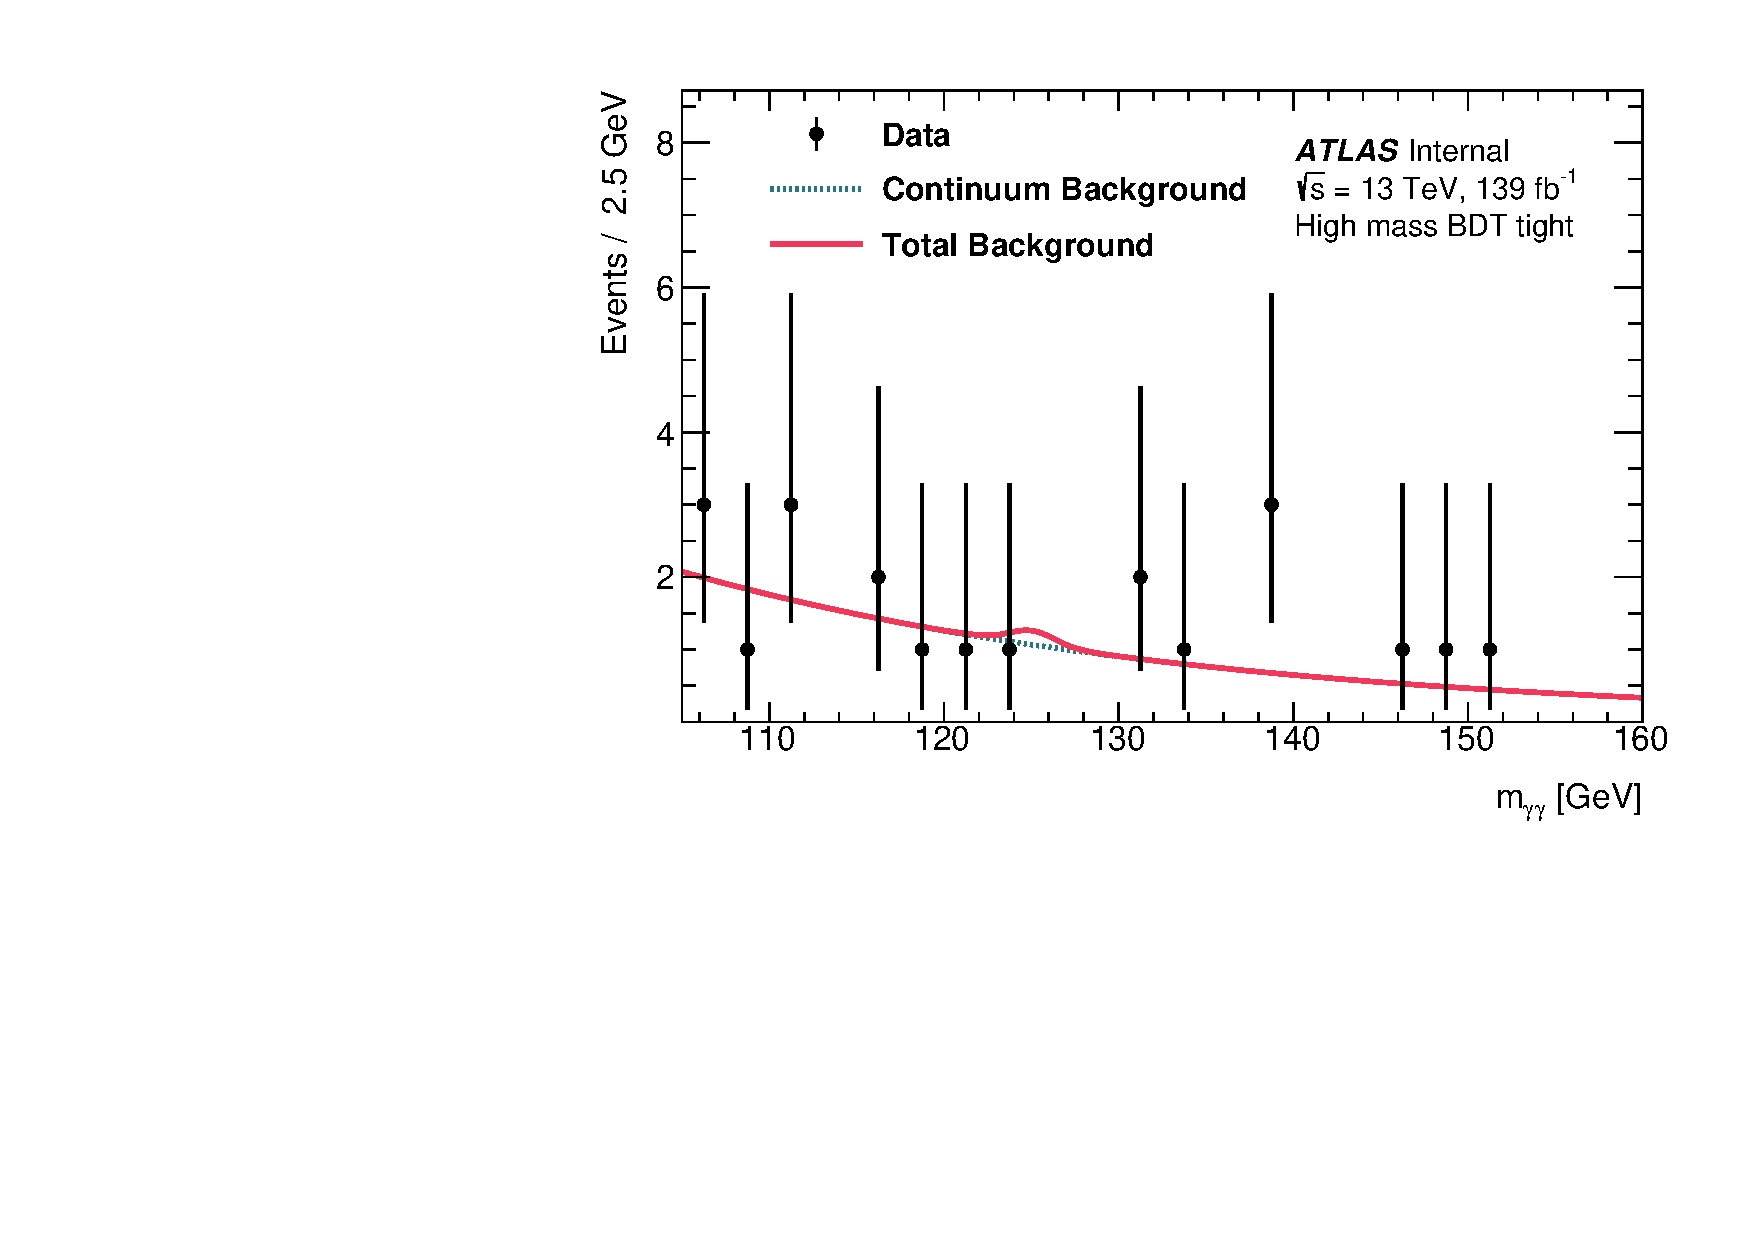
\includegraphics[width=.5\textwidth]{Ch5/Img/figures_Results_unweighted_yybb_SM_1_v2.pdf}}
    \subfloat[][Low mass, BDT tight ]{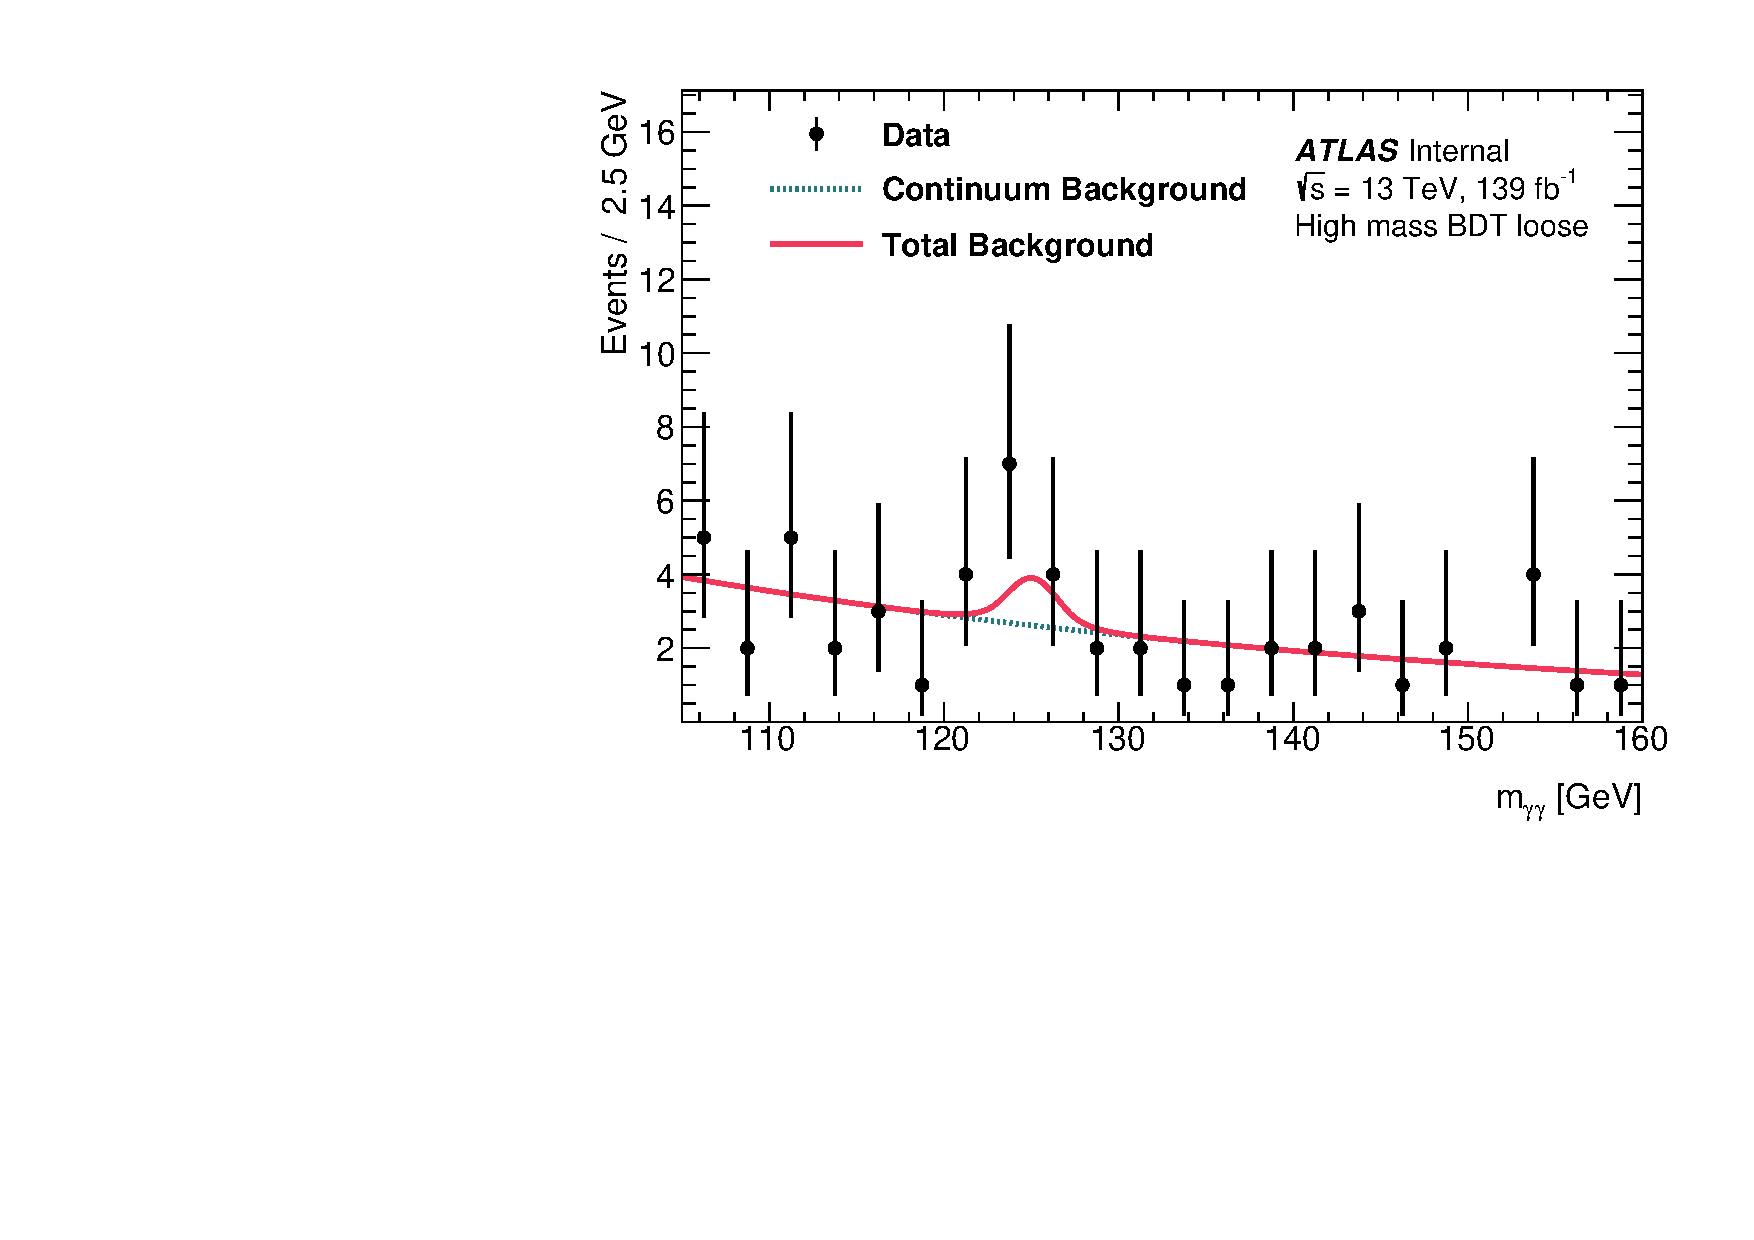
\includegraphics[width=.5\textwidth]{Ch5/Img/figures_Results_unweighted_yybb_SM_2_v2.pdf}} \\
    \subfloat[][High mass, BDT loose]{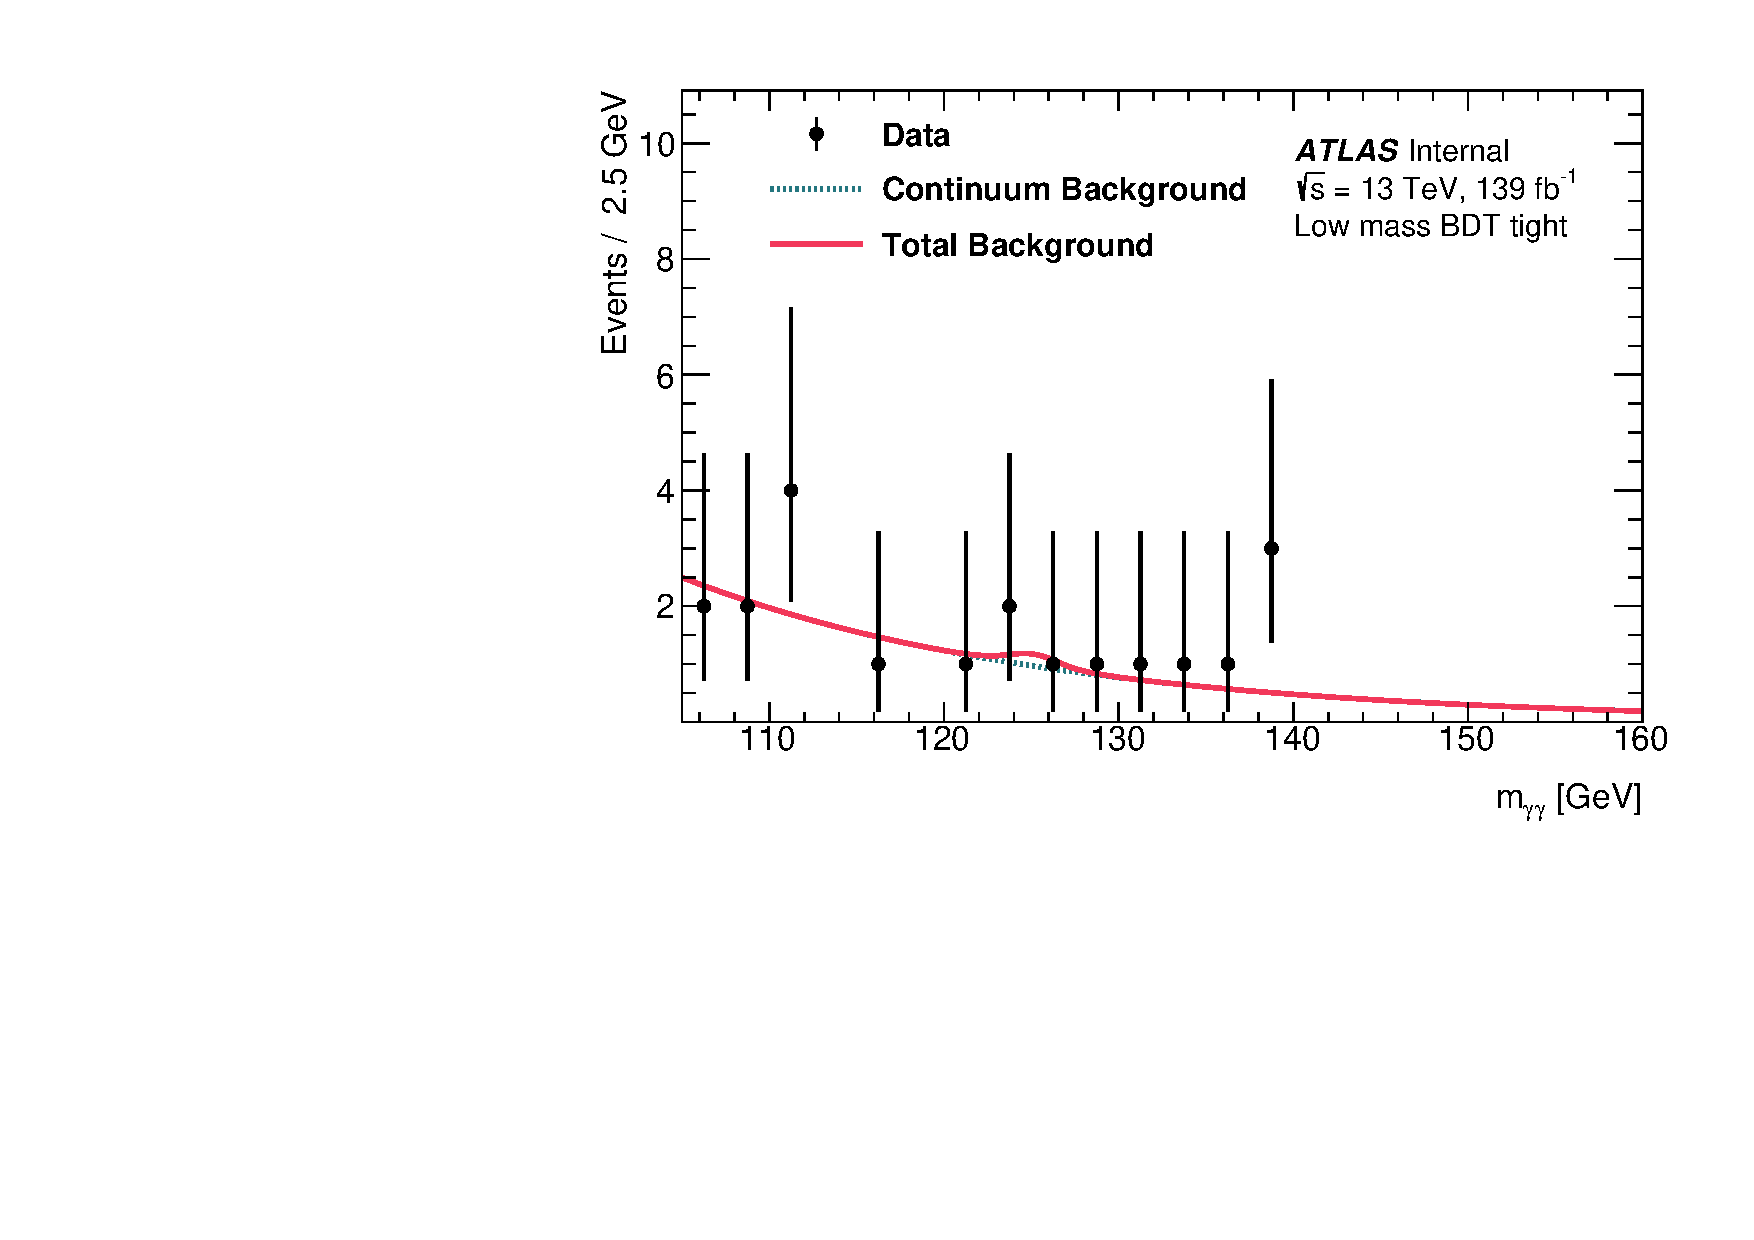
\includegraphics[width=.5\textwidth]{Ch5/Img/figures_Results_unweighted_yybb_BSM_1_v2.pdf}}
    \subfloat[][Low mass, BDT loose ]{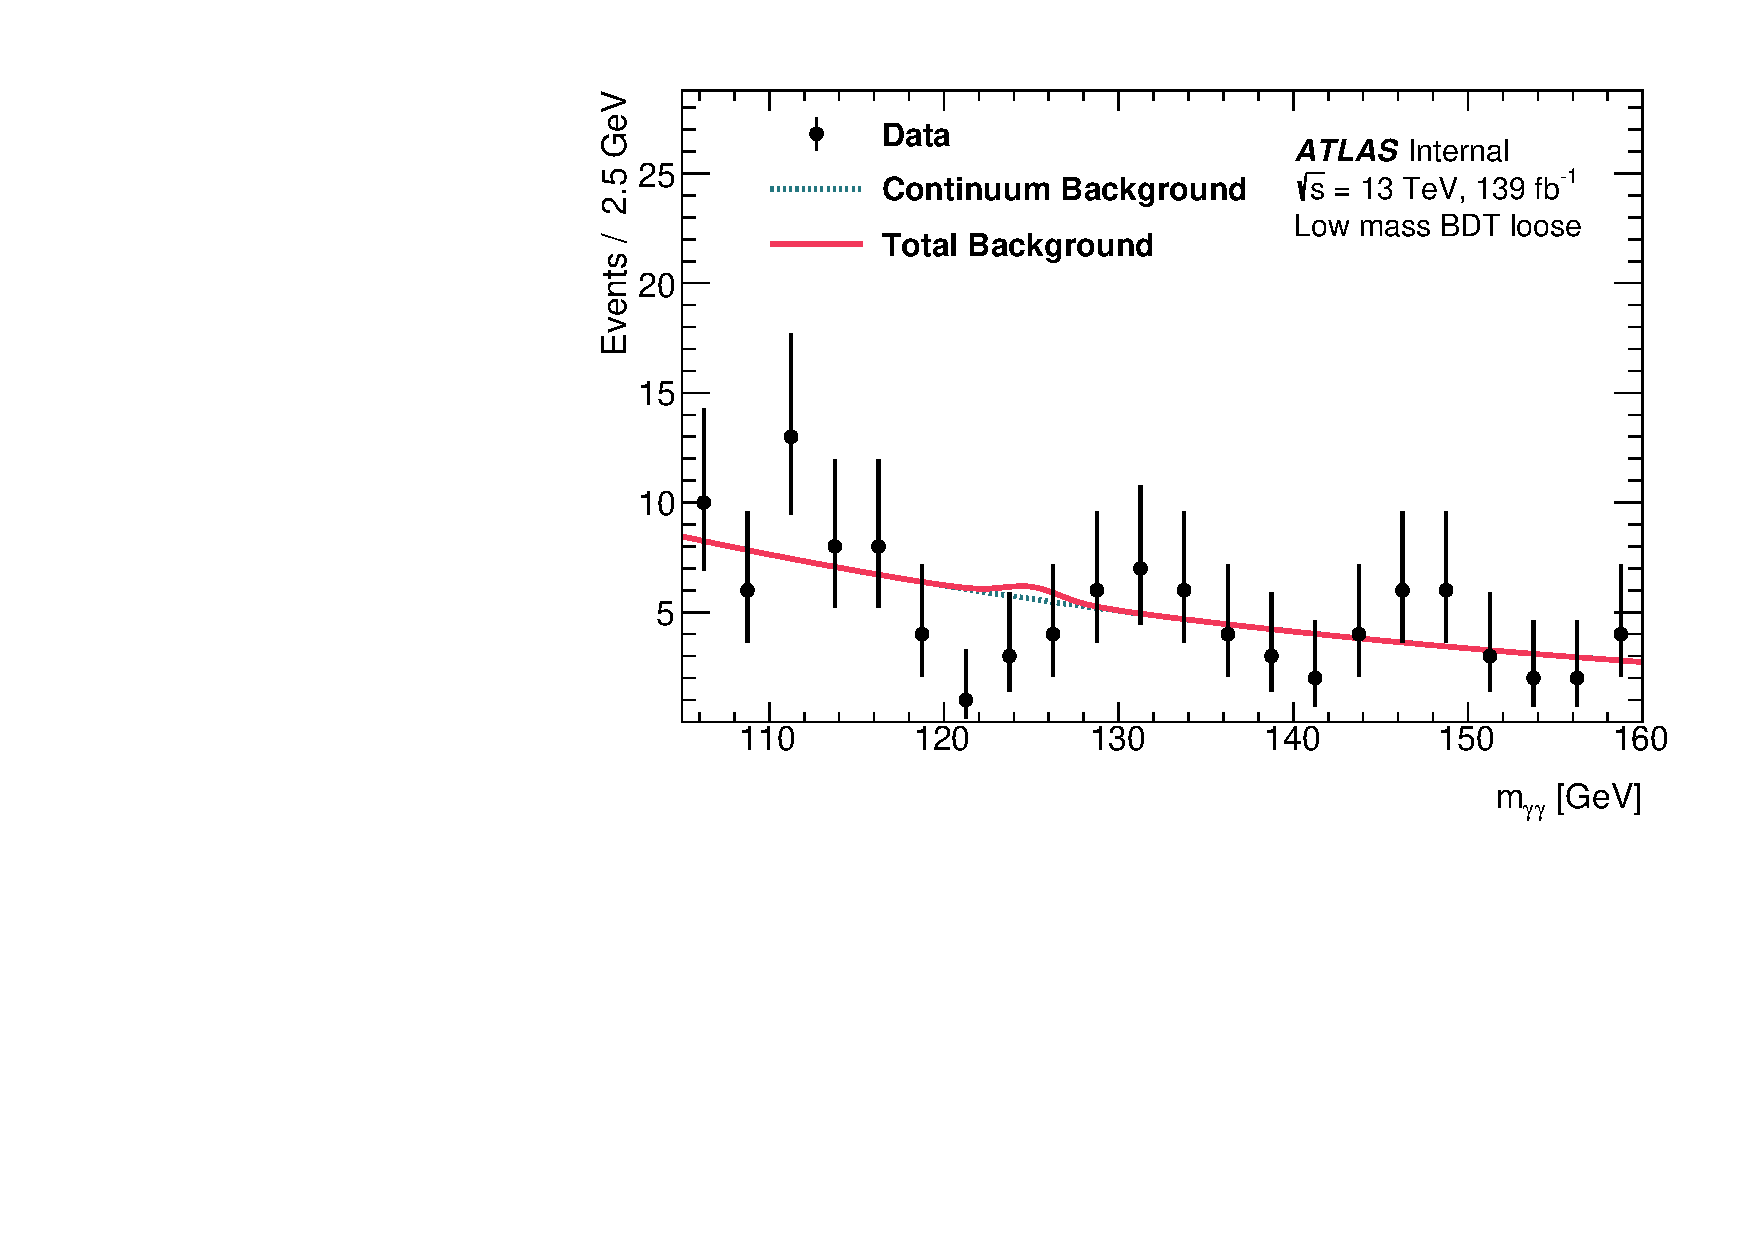
\includegraphics[width=.5\textwidth]{Ch5/Img/figures_Results_unweighted_yybb_BSM_2_v2.pdf}}
    \caption{The data are compared to the background-only fit for the four BDT categories. Both the continuum background and the background from single Higgs boson production are considered.}
    \label{fig:HHyybb:Results:Fit:myy}
\end{figure}
The number of the observed and expected events in each category is summarized in Table  \ref{fig:HHyybb:Results:Fit:NEvt}.
\begin{table}[]
\centering
\begin{tabular}{ccccc}
\hline \hline
& High mass & High mass & Low mass & Low mass \\
& BDT tight & BDT loose & BDT tight & BDT loose \\
\hline
Continuum & $4.9 \pm 1.1$ & $9.5 \pm 1.5$ & $3.7 \pm 1.0$ & $24.9 \pm 2.5$ \\
\hline
Single Higgs & $0.670 \pm 0.032$ & $1.57 \pm 0.04$ & $0.220 \pm 0.016$ & $1.39 \pm 0.04$ \\
$\mathrm{ggF}$ & $0.261 \pm 0.028$ & $0.44 \pm 0.04$ & $0.063 \pm 0.014$ & $0.274 \pm 0.030$ \\
$t \bar{t} H$ & $0.1929 \pm 0.0045$ & $0.491 \pm 0.007$ & $0.1074 \pm 0.0033$ & $0.742 \pm 0.009$ \\
$Z H$ & $0.142 \pm 0.005$ & $0.486 \pm 0.010$ & $0.04019 \pm 0.0027$ & $0.269 \pm 0.007$ \\
Rest & $0.074 \pm 0.012$ & $0.155 \pm 0.020$ & $0.008 \pm 0.006$ & $0.109 \pm 0.016$ \\
\hline SM HH (\kl = 1) & $0.8753 \pm 0.0032$ & $0.3680 \pm 0.0020$ & $(49.4 \pm 0.7) \cdot 10^{-3}$ & $(78.7 \pm 0.9) \cdot 10^{-3}$ \\
$\quad \mathrm{ggF}$ & $0.8626 \pm 0.0032$ & $0.3518 \pm 0.0020$ & $(46.1 \pm 0.7) \cdot 10^{-3}$ & $(71.8 \pm 0.9) \cdot 10^{-3}$ \\
VBF & $0.01266 \pm 0.00016$ & $0.01618 \pm 0.00018$ & $(3.22 \pm 0.08) \cdot 10^{-3}$ & $(6.923 \pm 0.011) \cdot 10^{-3}$ \\
\hline BSM HH (\kl = 10) & $6.36 \pm 0.05$ & $3.691 \pm 0.038$ & $4.65 \pm 0.04$ & $8.64 \pm 0.06$ \\
\hline Data & 2 & 17 & 5 & 14 \\
\hline \hline
\end{tabular}
\caption{Expected and observed numbers of events in the signal region ([120, 130] GeV) for the four BDT categories. The uncertainties on the continuum background are those arising from the fitting procedure. The uncertainties on the single Higgs boson and Higgs boson pair productions are from MC statistical error.}
\label{fig:HHyybb:Results:Fit:NEvt}
\end{table}

\subsection{Cross-section limits and \kl constrain}
\label{HHyybb:Results:Xsec}
 Since no significance excess over the SM prediction is found, exclusion limits at 95\% CL are claimed on the Higgs boson pair production cross section for each \kl as described in Section $\ref{HHyybb:Stat}$. The upper limits obtained for the Higgs boson production cross section $\sigma_{HH}$ in the ggF + VBF production modes is 140 fb were expecting 180 fb. As a multiple of the SM production cross-section, the observed limit is 4.1 times the SM prediction and the expected limit of 5.5 times the SM prediction. \\

As no HH event is observed, the constraint on the Higgs self coupling is derived from the cross-section limit scan versus \kl by taking the inter-section between the theoretical prediction and the measured cross section, as shown in Figure \ref{fig:HHyybb:Results:Xsec:Limit}. The observed constraint is -1.5 $<$ \kl $<$ 6.7, while the expected constraint is -2.4 $<$ \kl $<$ 7.7 obtained assuming \kl = 1. Effects from BSM scenario on the single Higgs cross section and Higgs boson branching ratio are neglected. The couplings of Higgs boson to other particles are set to their SM values \cite{Higgs_80ifb}. In addition to the constraint a measurement of \kl is performed by floating \kl in the fit and assuming SM prediction, the best-fit \kl is $2.7^{+2.1}_{-2.2}$ which is near to \kl with the minimum HH cross-section. The likelihood scan as a function of \kl is shown in Figure \ref{fig:HHyybb:Results:Xsec:LH}.
\begin{figure}[ht]
    \centering
    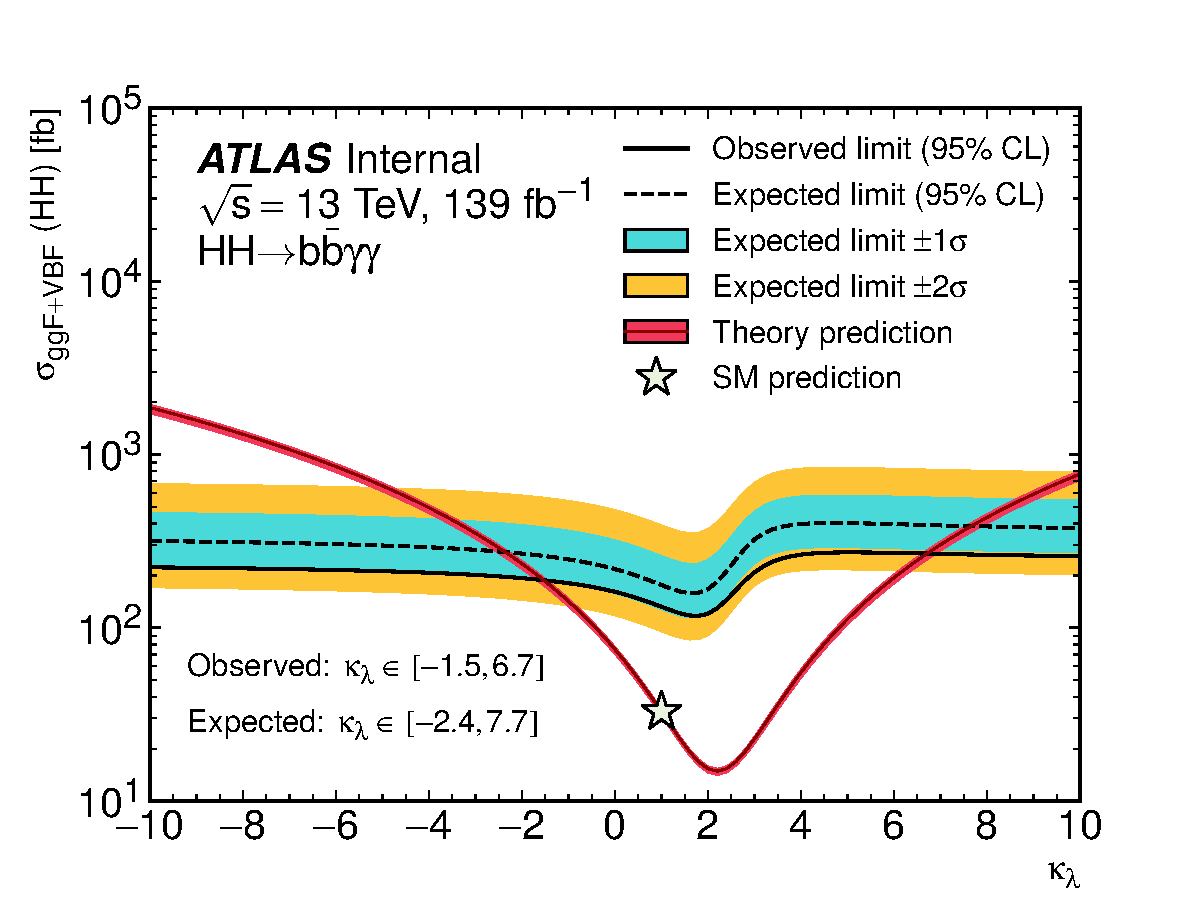
\includegraphics[width=0.5\textwidth]{Ch5/Img/figures_Results_kappa_lambda_scan.pdf}
    \caption{Observed and expected limits at 95\% CL on the cross section of non-resonant Higgs boson pair production as a function of the Higgs boson self-coupling modifier $\kappa_{\lambda}= \lambda_{HHH}/\lambda^{\textrm{SM}}_{HHH}$. The $\pm 1\sigma$ and $\pm 2\sigma$ bands show the variations on the expected limit due to statistical and systematic uncertainties. The theory prediction curve represents the scenario where all parameters and couplings are set to their SM values except for \kl. The uncertainty band of the theory prediction curve shows the cross section uncertainty.}
    \label{fig:HHyybb:Results:Xsec:Limit}
\end{figure}

\begin{figure}[ht]
    \centering
    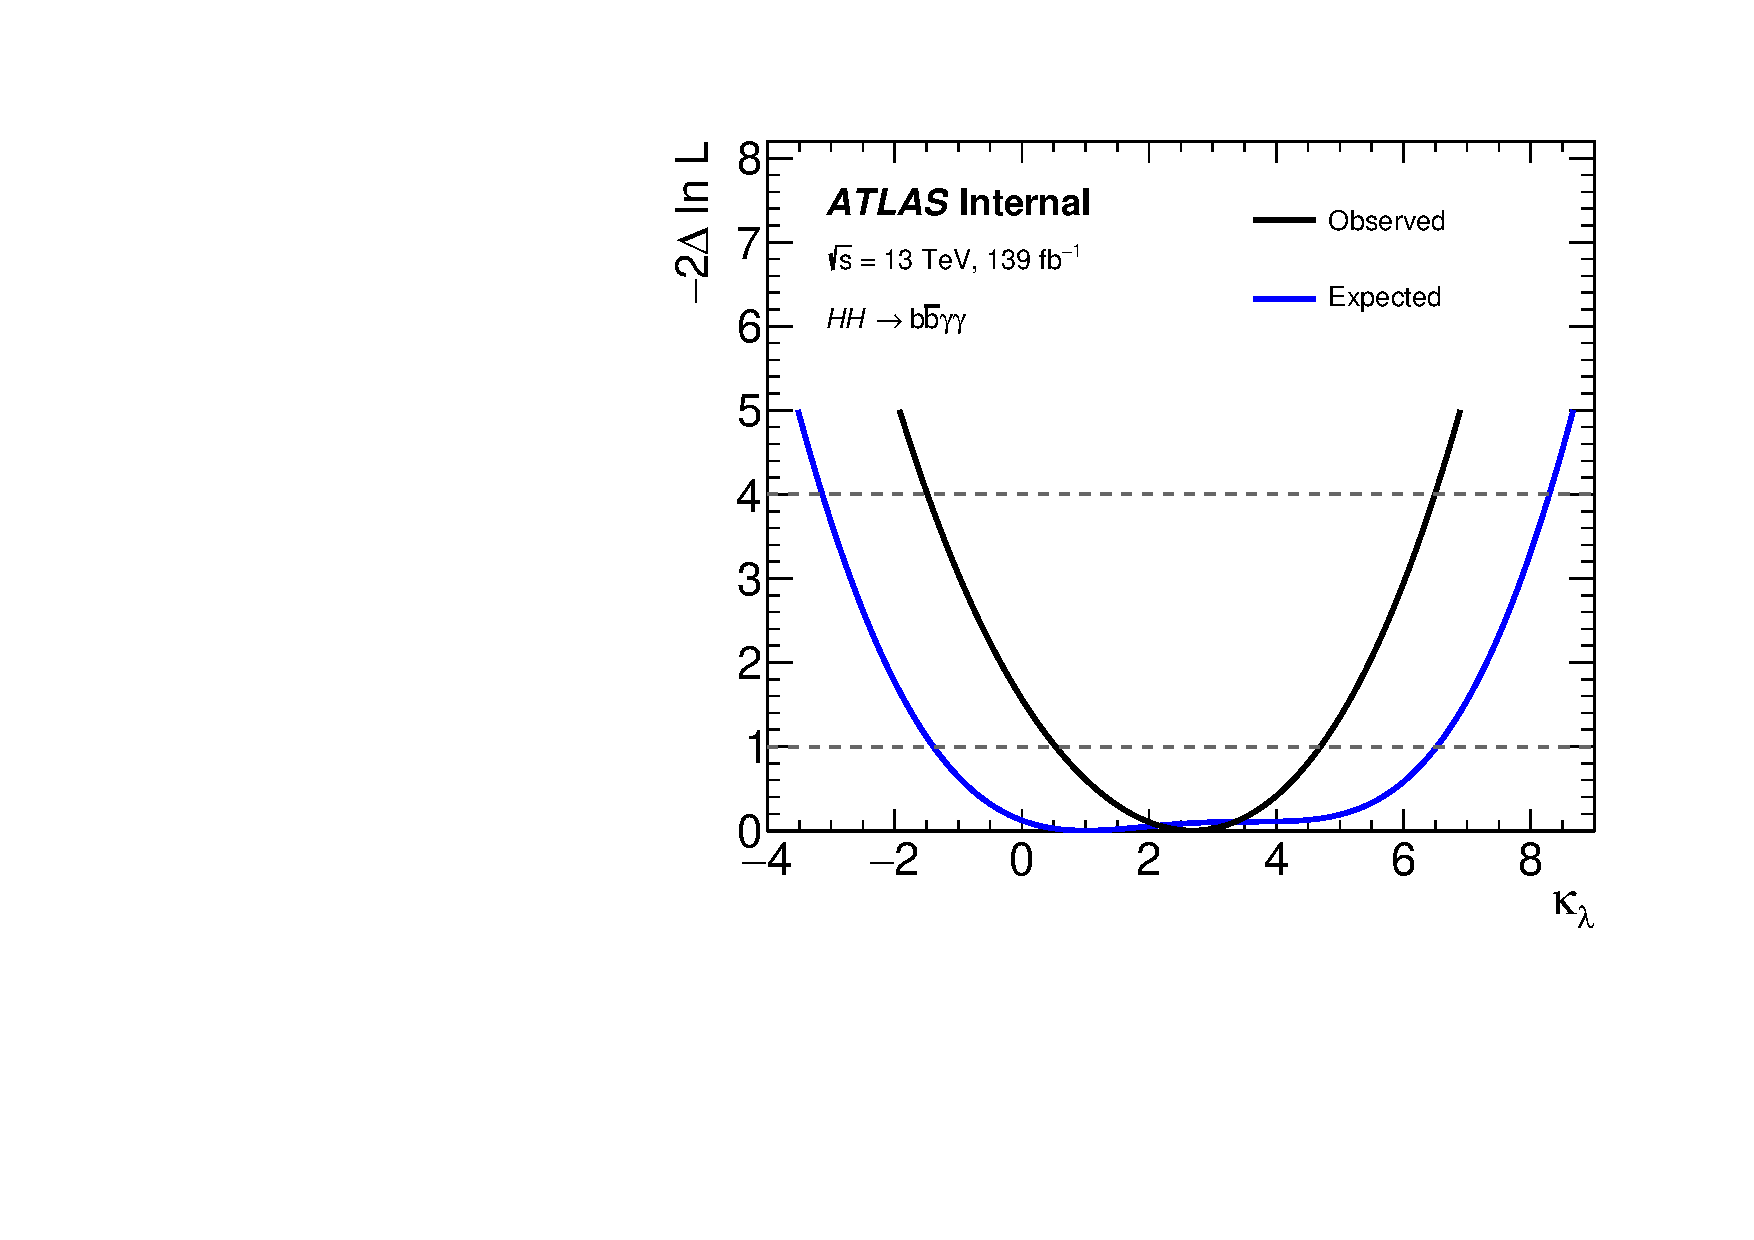
\includegraphics[width=0.5\textwidth]{Ch5/Img/figures_Results_scan_hhyybb_kl.pdf}
    \caption{The likelihood function as a function of \kl, with $\mu = $  1. The observed 68\% and 95\% CL ranges are [0.5, 4.7] and [-1.4, 6.5] respectively, while the expected are ([-1.4, 6.4] and [-3.1, 8.2].}
    \label{fig:HHyybb:Results:Xsec:LH}
\end{figure}

Table \ref{tab:HHyybb:Results:Xsec:Sys} shows the impact of the systematic uncertainties on the upper limit on $\mu$. The dominant systematic after the statistical uncertainties are related to the spurious signal and the photon energy scale (PES) uncertainties. As mentioned in Section \ref{HHyybb:Syst:Exp}, the PES systematic is arising from the measurement of photon energy and its calibrated which is mainly affected by the cell non-linearity, additional passive material in front of the calorimeter. The bias due to background function choice leads to the large spurious uncertainties and mainly dominated by the statistical fluctuations of the MC continuum background statistics used in the spurious signal test. Since generating of more MC events was however not possible in the time scale of the analysis, several attempts are done to improve the continuum statistics and reduce statistical fluctuation. The Gaussian Process Regression (GPR) \cite{GPR} is used to smooth and reduce fluctuations in the \myy distribution, this method reduces the $N_{SS}$ by 84\%. Increasing statistics by inverting the $b$-tagging requirements reduces the systematic on $\mu$ by $\sim$ 3\%. Since the analysis is statistically dominated, the global significance may not improve significantly, thus these improvement are not included.  
\begin{table}[ht]
    \centering
    \begin{tabular}{ccc}
\hline \hline 
Source & Type & Relative impact in \%  \\
\hline Experimental & & \\
\hline Photon energy scale & Norm. + Shape & 5.2  \\
Photon energy resolution & Norm. + Shape & 1.8  \\
Flavor tagging & Normalization & 0.5  \\
\hline Theoretical & & \\
\hline Heavy flavor content & Normalization & 1.5  \\
Higgs boson mass & Norm. + Shape & 1.8  \\
PDF+ $\alpha_{\mathrm{s}}$ & Normalization & 0.7  \\
\hline Spurious signal & Normalization & 5.5 \\
\hline \hline
\end{tabular}
    \caption{Breakdown of the dominant systematic uncertainties. Only systematic uncertainties with an impact of at least 0.5\% are shown. Uncertainties of Norm. + Shape type have effects on both the yield and the parameters of the functional form, the rest of uncertainties affects only the yields.}
    \label{tab:HHyybb:Results:Xsec:Sys}
\end{table}

\section{Comparison to 36 \ifb results}
\label{HHyybb:36ifb}

\section{Comparison to CMS \HHyybb results}
\label{HHyybb:CMS}